\documentclass[10pt,letterpaper]{article}
\usepackage[T1]{fontenc}
\usepackage[utf8]{inputenc}
\usepackage{lmodern}
\usepackage[margin=0.88in]{geometry}
\usepackage{microtype}
\usepackage{amsmath,amssymb,mathtools}
\usepackage{graphicx}
\usepackage{booktabs,tabularx,array}
\usepackage{enumitem}
\usepackage[font=small,labelfont=bf]{caption}
\usepackage{float}
\usepackage{hyperref}
\def\UrlBreaks{\do\/\do-\do\_\do\.}
\hypersetup{
  colorlinks=true,
  linkcolor=black,
  citecolor=black,
  urlcolor=blue,
  pdftitle={From Shared Weights to Head-Orthogonal Fibers: Virtual Depth, Head-Readable Staircases, and Post-Stall Search in Looped Transformers},
  pdfauthor={Patrick Dugan}
}
\setlength{\parindent}{1.1em}
\setlength{\parskip}{0.16em}
\setlist[itemize]{topsep=3pt,itemsep=1.5pt,leftmargin=*}
\renewcommand{\arraystretch}{1.12}

\newcommand{\LoopT}{\textsc{Loop-T}}
\newcommand{\FFU}{\textsc{FF-U}}
\newcommand{\EM}{\ensuremath{\mathrm{EM}}}
\newcommand{\IIA}{\ensuremath{\mathrm{IIA}}}
\newcommand{\DEF}{\ensuremath{\mathrm{DEF}}}
\newcommand{\cur}{\operatorname{cur\_node}}
\newcommand{\Gprop}{G_{\mathrm{prop}}}
\newcommand{\Phead}{P_{\mathrm{head}}}

\title{\bfseries From Shared Weights to Head-Orthogonal Fibers:\\[0.30em]
Virtual Depth, Head-Readable Staircases, and\\[0.14em]
Post-Stall Search in Looped Transformers}
\author{Patrick Dugan}
\date{November 2026\\[0.2em]\normalsize Unified synthesis across seven studies: \texttt{VPD}, \texttt{HUG-CAL-02}, \texttt{RMP}, \texttt{LOOPSCOPE-01}, \texttt{ARG-02}, \texttt{LOOPSCOPE-02}, and \texttt{LOOPSCOPE-03}}

\begin{document}
\maketitle
\vspace{-0.70em}

\begin{abstract}
\noindent
Weight-tied transformers reuse identical parameters across sequential passes, yet parameter sharing spans distinct computational regimes whose capability gains, failure modes, and latent-state monitorability differ sharply. Synthesizing seven studies across five experimental arcs—pretrained looped language models (\texttt{Nanbeige4.2-3B}, \texttt{Huginn-0125}), controlled algorithmic loopers (\LoopT, \texttt{LoopedChase}, \texttt{Lean-CGRT}), untied baselines (\FFU, \texttt{Qwen3.5-4B-Base}, \texttt{Qwen3-4B-Instruct}), and 7M-parameter convergent Tiny Recursive Models (\texttt{TRM})—we separate weight sharing into three mechanistic regimes and audit hidden-state computation via conditional refill, state-transplant \texttt{Resume} tests, and enforced path independence. First, two-pass language models implement \emph{fixed-pass virtual depth}: \texttt{Nanbeige4.2-3B} routes SwiGLU inputs through layer-selectively distinct singular subspaces across passes (mean top-64 SVD usage correlation $\bar{r}=0.355$; $r=0.085$ at \texttt{L12.mlp.down\_proj}) and rotates downstream perturbation directions when loop-boundary state is carried rather than reset, while discrete Top-32 sparse autoencoder support switches limit intervention-change fidelity ($F_\Delta > 0$ in $1/12$ second-pass \texttt{L22} edits despite Muon lifting state explained variance from $-0.180$ to $+0.453$). Across pointer chasing, 168-case finite-group composition (\texttt{ARG-02}: $65/168 = 38.7\%$ at native $t=2$, $76/168 = 45.2\%$ at $t=4$ [$p=0.080$], $71/168 = 42.3\%$ at $d^*=8$ [$p=0.61$]), and deductively stratified $9\times 9$ Sudoku (\texttt{LOOPSCOPE-02}), \texttt{Nanbeige4.2-3B} fails its registered recurrent gate (\texttt{H2a} $p=0.097$) and trails untied \texttt{Qwen3.5-4B-Base} on immediate single-cell elimination (\texttt{S1}: $11/64$ vs.\ $30/64$; overall $0.129$ vs.\ $0.211$, $p=0.0031$) while both sit near the $1/9 \approx 0.111$ uniform floor on multi-step strata (\texttt{S2--S4}). Second, multi-iteration and truncated-BPTT loopers exhibit \emph{dynamical settling and cache-dominated staircases—subject to a readout blind spot}: activation-matched input rotations on \texttt{Huginn-0125} (\texttt{HUG-CAL-02}; trained with random-init warmup and $k=8$ truncated BPTT) eliminate apparent late-iteration SVD specialization ($\pm 0.0065$ nats), motivating \emph{Transported Component Attribution} (\texttt{TCA}), which separates dynamical fragility from closed-form directional specificity in one backward pass ($\rho=0.75$ across 480 \texttt{Huginn} conditions) and exposes an observational Lyapunov contrast between multi-step BPTT and 1-step detached equilibrium gradients ($F_1/F_6 = 1{,}808.4$ across 126 core calls despite $0.303\times$ finite kick contraction, alongside $22.04\%$ read-specific components). On Markovian pointer chains, moderate intermediate supervision ($\lambda=0.1$) achieves $1.000$ depth-9--16 extrapolation with zero trajectory-residual cost across $3/3$ seeds, whereas dense supervision ($\lambda=1.0$) still routes $+3.06$ and $+5.46$ loops of active hop state through $\ker(\texttt{lm\_head})$ in $2/3$ seeds—instantiating Sharma and Vu's \cite{sharma2026dense} readout blind spot. Third, building on \texttt{HRM}/\texttt{TRM}'s coupled $(z_H, z_L)$ proposal-and-scratchpad design \cite{wang2025hrm,jolicoeur2025trm}, a 7M Sudoku \texttt{TRM} (336 core calls) solves $88.3\%$ of \texttt{items256} and $100\%$ of \texttt{bench100} ($71.9\%$ and $92.0\%$ on an independent replication checkpoint), commuting with exact propagation before stall ($\mathrm{AUC}=1.000$), while differential probes show $(I-\Phead)z_H$ tracks cell-flip and conflict-resolution history rather than a hidden tabu list (runner-up visible logits beat $\ker(\texttt{lm\_head})$ at recovering just-refuted digits). Decomposing full state into head-readable $V_t$, $(x,V_t)$-predictable cache $C_t = \hat{H}_\theta(x,V_t)$ across both $(I-\Phead)z_H$ and $z_L$, and residual $R_t = H_t - C_t$ (\texttt{LOOPSCOPE-03}) shows that joint $V$-only erasure drops stalled solve to $0.617$ and $0.519$ ($33.3\%$--$44.8\%$ limit cycles at $s=64$), propagation boards are pure cache ($73/73$ on both checkpoints), and \emph{$R_t$ is causally active—with checkpoint-dependent sign—only on stalled boards}. Scaling \texttt{C5} training data $9\times$ ($N=100 \to 8{,}100$ disjoint boards) raises held-out $R^2$ from $0.844 \to 0.915$ ($0.689 \to 0.837$ replication), narrowing every-step closed-loop primary stalled loss to $-4.9$~pp ($s=16$) and $-7.1$~pp ($s=64$) while boosting replication $+16.9$~pp above clean ($0.590 \to 0.760$); refilling every $m \ge 2$ steps ($0.874$--$0.896$, $p \ge 0.289$) or single-transplant \texttt{Resume} on clean states yields $0.0$ median loop delay across unselected mutual solvers on primary ($\Delta\texttt{NeverLock} \le +2.2$~pp) versus $-2.0$ to $-4.0$ median loops ($p \le 0.0014$) and $-10.5$~pp \texttt{NeverLock} ($p=0.017$) on unresolved replication boards (while our registered flip-correlation gate failed at $\rho=0.198 < 0.25$). Finally, scoring \emph{unconditional} fork agreement across $K=8$ starts (avoiding unique-Sudoku solved-only tautology) explains why replicating Kubo et al.'s \cite{kubo2026cvoting} \texttt{C-voting} lifts stalled solve ($0.836 \to 0.940$; $0.656 \to 0.858$) and confirms Anil et al.\ \cite{anil2022path}: conditional refill enforces path independence ($\mathrm{PI}_{\mathrm{cell}}(64)$: $0.603 \to 0.937$ at $\sigma=1.0$), rescuing the path-dependent checkpoint ($+39.1$~pp in the lowest-PI quartile) while slightly hurting the already path-independent one only under every-step closed-loop drift.
\end{abstract}

\section{Introduction: Three Regimes of Weight Sharing}\label{sec:intro}

A weight-tied transformer applies identical block parameters $\theta$ across $T$ sequential passes \cite{dehghani2019universal,giannou2023looped,saunshi2025latent,geiping2025huginn,wang2025hrm,jolicoeur2025trm,li2026deeploop}. Because parameter identity no longer indexes computational depth, two questions govern capability and interpretability in recurrent-depth architectures:
\begin{enumerate}[topsep=3pt,itemsep=2pt]
  \item \textbf{Capability triangulation:} When does reusing $\theta$ across passes yield multi-step algorithmic or combinatorial reasoning beyond an untied transformer, and what dynamical invariants separate fixed-pass stage pipelines from convergent recursive solvers?
  \item \textbf{Latent monitorability:} When can intermediate computation be audited directly through the output readout head $\Phead$, when does state orthogonal to the readout ($\ker(\texttt{lm\_head})$) carry causal search information, and is that head-orthogonal state opaque to linear probes or merely invisible to token logits?
\end{enumerate}

Our September 2026 study of the pretrained two-pass language model \texttt{Nanbeige4.2-3B} \cite{nanbeige2026model,dugan2026vpd} examined shared MLP matrices via multipass vector parameter decomposition (\texttt{VPD}) \cite{braun2025apd} and shared Top-32 sparse autoencoders (\texttt{SAE}s) \cite{bricken2023monosemanticity,gao2024scaling} across \texttt{ARC-AGI-1}, \texttt{ARC-AGI-2}, and the \texttt{logic} and \texttt{math} subsets of \path{PrimeIntellect/INTELLECT-3-RL} \cite{primeintellect2025intellect3}. That study found sharp terminal-layer pass divergence, showed that Muon-hybrid optimization \cite{jordan2024muon,dugan2026muonsae} rescues second-pass state reconstruction without rescuing intervention-change fidelity, and proved via a 44-layer embedding-reset control that carrying loop-boundary state rotates downstream perturbation directions. Yet it left open whether two-pass reuse buys multi-step deduction, whether per-iteration weight-ablation asymmetries reflect specialized factors or dynamical sensitivity, and where the boundary lies between head-readable iteration and head-orthogonal state.

Over the subsequent ten weeks, foundational equilibrium-model priors and concurrent 2026 looped-transformer studies established key properties of recurrent computation while leaving these questions open (Table~\ref{tab:literature}). Earlier, Anil et al.\ \cite{anil2022path} connected out-of-distribution iteration scaling in equilibrium models to \emph{path independence}—convergence to the same fixed point from arbitrary initializations, whereas path-dependent models degrade once test iterations exceed the training budget—and Wang et al.\ (\texttt{HRM}) \cite{wang2025hrm} and Jolicoeur-Martineau (\texttt{TRM}) \cite{jolicoeur2025trm} introduced coupled dual-state recurrence $(z_H, z_L)$ (designating $z_H$ as the current proposed solution and $z_L$ as a latent reasoning scratchpad updated under 1-step equilibrium gradients) to support iterative backtracking on hard puzzles. Concurrently, Kubo et al.\ \cite{kubo2026cvoting} introduced confidence-based voting (\texttt{C-voting}) across randomly initialized latent trajectories at test time, demonstrating that multi-start selection exploits outcome variance across initializations; Sharma and Vu \cite{sharma2026dense} identified the \emph{readout blind spot}—showing that even dense per-step intermediate logit supervision leaves $\ker(\texttt{lm\_head})$ unconstrained, producing a visibility--activity mismatch when active computation routes off-axis; Blayney et al.\ \cite{blayney2026mechanistic} analyzed cyclic fixed points and the stabilizing roles of input injection and normalization; Kaissis et al.\ \cite{kaissis2026sdi} introduced Step-Decomposed Influence (\texttt{SDI}) to decompose TracIn training-data influence across BPTT iterations; Wu, Hu, and Zhang \cite{wu2026shared} introduced linear \texttt{J}-steering on frozen loops; Sesodia et al.\ \cite{sesodia2026inside} demonstrated matched-training advantages and iteration-budget staircases in weight-tied transformers; and Olszowiec et al.\ \cite{olszowiec2026monitoring} showed across eight looped language models that hidden-state stability depends strongly on per-step input re-injection (complementing Geiping et al.'s \cite{geiping2025huginn} random-init warmup and $k=8$ truncated BPTT in \texttt{Huginn-0125}).

\begin{table}[t]
\centering
\small
\begin{tabularx}{\linewidth}{@{}l>{\raggedright\arraybackslash}p{0.31\linewidth}>{\raggedright\arraybackslash}X@{}}
\toprule
Prior / concurrent study & Principal contribution & Complementary contribution in this synthesis \\
\midrule
Anil et al.\ \cite{anil2022path}; Kubo et al.\ \cite{kubo2026cvoting} & Path independence governs OOD iteration scaling; \texttt{C-voting} selects confident multi-init runs & Replicates \texttt{C-voting} on \texttt{TRM} ($0.836{\to}0.940$; $0.656{\to}0.858$); shows conditional refill enforces path independence ($\mathrm{PI}_{\mathrm{cell}}{:}\ 0.603{\to}0.937$) and rescues OOD scaling \\
Wang et al.\ (\texttt{HRM}) \cite{wang2025hrm}; \texttt{TRM} \cite{jolicoeur2025trm} & Dual $(z_H, z_L)$ proposal + scratchpad states, 1-step gradients, puzzle backtracking & Isolates $z_H \times z_L$ mutual backup ($33\%$--$45\%$ limit cycles under joint $V$-only erasure) and $1{,}808\times$ detached-ACT tangent inflation \\
Sharma \& Vu \cite{sharma2026dense} & Dense logit supervision leaves $\ker(\texttt{lm\_head})$ blind spot & Instantiates blind spot on $\lambda{=}1.0$ \texttt{LoopedChase} ($+3.06, +5.46$ off-axis loops vs.\ $0.00$ at $\lambda{=}0.1$) and \texttt{Post-RMSNorm} radial norms \\
Blayney et al.\ \cite{blayney2026mechanistic} & Cyclic fixed points and normalization / injection effects in looped LMs & Isolates $33.3\%$--$44.8\%$ periodic visible-board limit cycles under $V$-only erasure and $25.1\%$ clean limit cycles halved by cache refill \\
Kaissis et al.\ (\texttt{SDI}) \cite{kaissis2026sdi} & Decomposes TracIn data influence across BPTT loops via $\sum \delta_s \otimes a_s$ & Analytical caution: detached-ACT tangent Jacobians inflate step-1 norms by $1{,}808\times$ ($6{,}400\times$ max); \texttt{TCA} cancels $\|A_s\|$ via rotation nulls \\
Wu, Hu \& Zhang \cite{wu2026shared}; Sesodia et al.\ \cite{sesodia2026inside} & Linear \texttt{J}-steering, uneven logit steps, matched-training staircases & Quantifies SVD multiplexing ($\bar{r}{=}0.355$) vs.\ stationary reuse ($\bar{r}{=}0.992$), \LoopT\ vs.\ \FFU, and covariate-shift-free \texttt{Resume} delays \\
Geiping et al.\ \cite{geiping2025huginn}; Olszowiec et al.\ \cite{olszowiec2026monitoring} & Random-init warmup + $k{=}8$ trunc.\ BPTT (\texttt{Huginn}); re-injection stability & Splits hidden state into $(x,V_t)$-predictable cache $C_t$ ($99.94\%$ in \texttt{Huginn} at $t{=}32$; $R^2{=}0.915$ in \texttt{TRM} at $N{=}8{,}100$) vs.\ residual $R_t$ \\
\bottomrule
\end{tabularx}
\caption{Positioning relative to equilibrium path-independence theory, \texttt{HRM}/\texttt{TRM} state-role priors, and concurrent 2026 looped-transformer studies.}
\label{tab:literature}
\end{table}

Synthesizing seven studies across five experimental arcs—September \texttt{VPD} \cite{dugan2026vpd}, registered \texttt{Huginn-0125} calibration (\path{HUG-CAL-02} \cite{dugan2026hugcal}), controlled closed-loop mediation and compactification (\texttt{RMP} \cite{dugan2026rmp}, \path{LOOPSCOPE-01} \cite{dugan2026loopscope01}, \path{ARG-02} \cite{dugan2026arg02}), stratified $9\times 9$ Sudoku triangulation with head-orthogonal manifold controls (\path{LOOPSCOPE-02}), and three-ledger conditional refill, \texttt{Resume}, and enforced path-independence controls (\path{LOOPSCOPE-03} \cite{dugan2026loopscope01})—we establish three mechanistic regimes:
\begin{itemize}
  \item \textbf{Regime I — Fixed-Pass Virtual Depth (Section~\ref{sec:regime1}):} Without input re-injection, fixed $T=2$ \texttt{Nanbeige4.2-3B} routes nonlinear MLP activations through pass-divergent singular subspaces ($\bar{r}=0.355$) as a compressed 44-layer pipeline, failing stationarity admission for state-transplant tests and failing to contract perturbations ($6.9\times$ amplification) or clear multi-step deductive strata (note that in pretrained LMs, fixed $T=2$ depth and absence of input re-injection remain confounded because \texttt{Nanbeige4.2-3B} is both our sole Regime I model and our sole pretrained checkpoint without re-injection).
  \item \textbf{Regime II — Dynamical Settling and Cache-Dominated Staircases with a Readout Blind Spot (Sections~\ref{sec:fragility}--\ref{sec:regime2}, \ref{sec:loopscope03}):} In multi-step and truncated-BPTT loopers, apparent late-loop SVD specialization on \texttt{Huginn-0125} (trained with random-init warmup and $k=8$ truncated BPTT \cite{geiping2025huginn}) vanishes under activation-matched input rotations (\texttt{HUG-CAL-02}), formalized in one pass by \texttt{TCA}, while path-dependent hidden variance contracts to $0.06\%$ ($99.94\%$ input-conditioned cache) by $t=32$. On Markovian chains (\texttt{LoopedChase}), moderate per-loop supervision ($\lambda = 0.1$) yields $1.000$ OOD extrapolation, $\mathrm{AUC}=0.992$ belief commutation, $1.000$ all-token conditional-cache sufficiency, and $0.00$ residual loops across $3/3$ seeds—whereas dense $\lambda=1.0$ supervision routes $+3.06$ and $+5.46$ active loops through $\ker(\texttt{lm\_head})$ in $2/3$ seeds, instantiating Sharma and Vu's \cite{sharma2026dense} readout blind spot.
  \item \textbf{Regime III — Stationary Attractor Search and Enforced Path Independence (Sections~\ref{sec:regime3}--\ref{sec:loopscope03}):} Building on \texttt{HRM}/\texttt{TRM}'s $(z_H, z_L)$ architecture \cite{wang2025hrm,jolicoeur2025trm}, a 7M Sudoku \texttt{TRM} (336 core calls with input re-injection) iterates a stationary outer operator ($\bar{r}_{\mathrm{outer}}=0.992$) that contracts finite kicks ($0.303\times$) and splits state into head-readable $V_t$, $(x,V_t)$-predictable cache $C_t$, and trajectory residual $R_t$. Joint $V$-only erasure traps $33.3\%$--$44.8\%$ of stalled boards in periodic visible-board limit cycles at $s=64$, while propagation boards are pure cache ($73/73$ on both checkpoints). Across two checkpoints, $R_t$ is causally active—with opposite sign—strictly on stalled boards: scaling \texttt{C5} to $N=8{,}100$ disjoint boards ($R^2 = 0.915$ primary, $0.837$ replication) narrows every-step closed-loop primary loss to $-4.9$~pp ($s=16$) and $-7.1$~pp ($s=64$) (with $0.0$ median loop delay under single-step \texttt{Resume} and full recovery by periodic cadence $m \ge 2$) while lifting the strongly path-dependent replication checkpoint $+16.9$~pp above clean ($+19.1$~pp at $m=2$) by enforcing hidden-state path independence \cite{anil2022path}.
\end{itemize}

\paragraph{Provenance and archival discipline.} Pre-registered decision rules and post-hoc controls are kept strictly distinct: all pre-registered gates that returned \texttt{Not supported}, \texttt{Weak}, \texttt{Partially supported}, or failed sub-thresholds (\texttt{HUG-CAL-02}, \texttt{ARG-02} \texttt{H2a}, \texttt{LOOPSCOPE-02} \texttt{P1}--\texttt{P4}, and \texttt{LOOPSCOPE-03} \texttt{H3.3}'s failed $\rho = 0.198 < 0.25$ flip-correlation gate) are reported plainly without metric substitution. Because our development repository is private, all pre-registration files, verbatim registration commit patches (\texttt{1f205d67} and \texttt{b1ec7755}), evaluation reports, scripts, and JSON receipts for \texttt{LOOPSCOPE-02} and \texttt{LOOPSCOPE-03} are publicly mirrored in \url{https://github.com/MoralityLabAI/VPD/tree/main/output/supplements}, and archival snapshots \texttt{VPD} \texttt{v001}--\texttt{v013} and \texttt{papers/rmp\_looped\_mechinterp} remain unmodified.

\section{Regime I: Two-Pass Virtual Depth, Support Switching, and SVD Multiplexing}\label{sec:regime1}

We first examine \texttt{Nanbeige/Nanbeige4.2-3B} \cite{nanbeige2026model} (revision \texttt{451ed48c}), a pretrained decoder executing 22 shared transformer layers twice per forward pass ($T=2$, 44 executed layers) with a loop-boundary \texttt{RMSNorm} and \emph{no} re-injection of token embeddings before Pass 2 (making $T=2$ training depth and absence of re-injection co-occurring properties of this checkpoint; Section~\ref{sec:discussion}).

\subsection{Terminal Pass Divergence and the Muon SAE Fidelity Gap}

In \cite{dugan2026vpd}, a 64-component multipass \texttt{VPD} decomposition (\texttt{prime-20260906T204058Z-561}, capturing $\approx 2.2\%$ of squared weight norm at \texttt{mlp.down\_proj} of physical layers 12 and 22) and shared 6,144-latent Top-32 \texttt{SAE}s were evaluated on 18 reasoning trajectories (8 calibration, 10 held-out across 8 task groups) from \texttt{ARC-AGI-1}, \texttt{ARC-AGI-2}, and \path{PrimeIntellect/INTELLECT-3-RL} (\texttt{logic} and \texttt{math} subsets) \cite{primeintellect2025intellect3}. Residual-stream cosine similarity between Pass 1 and Pass 2 stays high at physical mid-layer \texttt{L12} ($0.799$--$0.869$) but drops sharply at terminal physical layer \texttt{L22} to $0.230$--$0.307$ ($0.184$--$0.229$ post-loop-norm), already within the prompt suffix before generation.

Fitting one shared Top-32 \texttt{SAE} across both passes under AdamW yielded negative held-out \texttt{L22} Pass-2 state explained variance ($\mathrm{EV} = -0.180$ on Q4 trajectories; $-0.535$ on BF16 intervention baselines, vs.\ $+0.830$ and $+0.763$ on Pass 1). Switching matrix parameters to Muon \cite{jordan2024muon,dugan2026muonsae} rescued static reconstruction ($\mathrm{EV} = +0.453$ Q4, $+0.312$ BF16 on Pass 2; $0.918$ and $0.942$ on Pass 1), yet failed to rescue \emph{intervention-change fidelity} for true shift $\Delta h = h_1 - h_0$ and reconstructed shift $\Delta \hat{h} = \hat{h}_1 - \hat{h}_0$ ($e(h)=h-\hat{h}$):
\begin{equation}
  F_\Delta \;=\; 1 - \frac{\|\Delta h - \Delta \hat{h}\|_2^2}{\|\Delta h\|_2^2}
  \;=\; 1 - \frac{\|e(h_1) - e(h_0)\|_2^2}{\|\Delta h\|_2^2}.
  \label{eq:fdelta}
\end{equation}
Muon improved \texttt{L22} Pass-2 $F_\Delta$ in $12/12$ conditions ($18/20$ nonzero \texttt{L22} conditions overall), but only $1/12$ exceeded zero ($+0.030$). Discrete Top-32 encoder support switches at $1$--$3$ of $80$ positions caused $93.3\%$--$99.6\%$ of change-mismatch energy; freezing baseline active support reduced a unit-write mismatch from $-52.367$ to $-0.000543$. A 44-layer \emph{embedding-reset control} replacing Pass-1 output with token embeddings matched 22-layer one-pass states bit-for-bit across 150 pairs and kept propagated \texttt{L12}$\to$\texttt{L22} Muon $F_\Delta$ positive ($+0.047$ to $+0.572$) versus negative under state carry ($-0.300$ to $-0.046$); crossing baselines with unit response directions confirmed that state carry rotates downstream Jacobian directions ($0.059/0.051$ carry vs.\ $0.354/0.377$ reset).

\subsection{Triangulating Pretrained Capability Across Pointer Chasing, Algebra, and Sudoku}

Unlike matched-training studies where weight-tied models outperform depth-matched untied baselines trained on the same corpus \cite{sesodia2026inside} (replicated in our controlled \LoopT\ vs.\ \FFU\ experiments in Section~\ref{sec:regime2}), comparing pretrained \texttt{Nanbeige4.2-3B} against untied \texttt{Qwen} checkpoints is observational across model families, parameter counts, and pretraining mixtures; it tests whether \texttt{Nanbeige}'s two-pass reuse exhibits iterative scaling at inference (Figure~\ref{fig:triangulation}, Table~\ref{tab:sudoku_triangulation}):
\begin{enumerate}[topsep=3pt,itemsep=2pt]
  \item \textbf{Pointer chasing (\texttt{Silico Stage 1}):} On 3-shot 16-node chains, \texttt{Nanbeige4.2-3B} scores $79.2\%$ at 1 hop (chance $6.25\%$) and $6.55\%$ ($131/2{,}000$) across depths 3--6, with Pass-1-only sensitivity on top \texttt{L22} \texttt{VPD} factors \texttt{(19, 9, 43)} ($-0.060$ to $-0.098$ nats on Pass 1; $0.000$ on Pass 2).
  \item \textbf{Finite-group composition (\texttt{ARG-02} Extension N1 \cite{dugan2026arg02}):} On $N=168$ held-out group trace items (\texttt{future@12}, dev-selected budget $d^*=8$ from 132 dev items), \texttt{Nanbeige4.2-3B} solves $44/168$ ($26.2\%$) at $t=1$, $65/168$ ($38.7\%$) at native $t=2$ ($+21$ items, McNemar $p=0.040$), $76/168$ ($45.2\%$) at OOD $t=4$ ($+11$ over $t=2$, $p=0.080$), and $71/168$ ($42.3\%$) at $d^*=8$ ($+6$ over $t=2$, $p=0.61$), compared with single-pass \texttt{Qwen3.5-0.8B} ($68/168 = 40.5\%$) and \texttt{Qwen3.5-2B} ($79/168 = 47.0\%$). Thus OOD loops $t=4,8$ show positive point-estimate gains over $t=2$ that do not reach statistical significance. Pre-registered recurrent mechanism gate \texttt{H2a}—requiring closed-loop $d^*=8$ ($71/168$) to significantly beat linear open-loop extrapolation $h_{\mathrm{open}}(t) = h(1) + (t-1)(h(1)-x)$ ($55/168 = 32.7\%$ at both $t=2$ and $t=8$)—failed ($+16$ items, $p=0.097$); donor-shuffled Pass-2 displacements scored $69/168$ ($41.1\%$, differing from clean $t=2$ on $6/168$ items), and $0.25\cdot\mathrm{RMS}$ kicks amplified by $2.8\times \to 3.9\times \to 6.9\times$ across loops $2, 4, 8$.
  \item \textbf{Stratified $9\times 9$ Sudoku (\texttt{LOOPSCOPE-02}):} Across 256 held-out \texttt{sudoku-extreme} boards stratified into $n=64$ per deductive round class of exact synchronous naked- plus hidden-single propagation $\Gprop$—\texttt{S1\_naked1} ($r=1$), \texttt{S2\_prop2} ($r=2$), \texttt{S3\_prop3plus} ($r\ge 3$), and \texttt{S4\_stalled} (zero singles anywhere on the board at round 0)—single-target-cell 3-shot accuracy is $25/256$ ($0.098$) at $t=1$, $33/256$ ($0.129$) at $t=2$ ($p=0.341$), and $23/256$ ($0.090$) at $t=8$ ($p=0.220$). Crucially, uniform digit guessing gives $1/9 \approx 0.111$ ($\pm 0.077$ two-SE sampling band at $n=64$): every \texttt{Nanbeige} stratum and the \texttt{S2--S4} strata of both \texttt{Qwen} models lie within sampling noise of this floor, so absence of loop scaling cannot be inferred from \texttt{S2--S4} alone. Instead, the entire advantage of untied \texttt{Qwen3.5-4B-Base} ($54/256 = 0.211$, McNemar $p=0.0031$) and pure-SDPA \texttt{Qwen3-4B-Instruct} ($65/256 = 0.254$) over \texttt{Nanbeige} ($t=2$) resides in immediate 1-round elimination \texttt{S1\_naked1} ($30/64 = 0.469$ and $36/64 = 0.562$ vs.\ $11/64 = 0.172$; on \texttt{S2--S4} combined, $24/192 = 0.125$ vs.\ $22/192 = 0.115$, $p=0.824$).
\end{enumerate}

\begin{figure}[t]
\centering
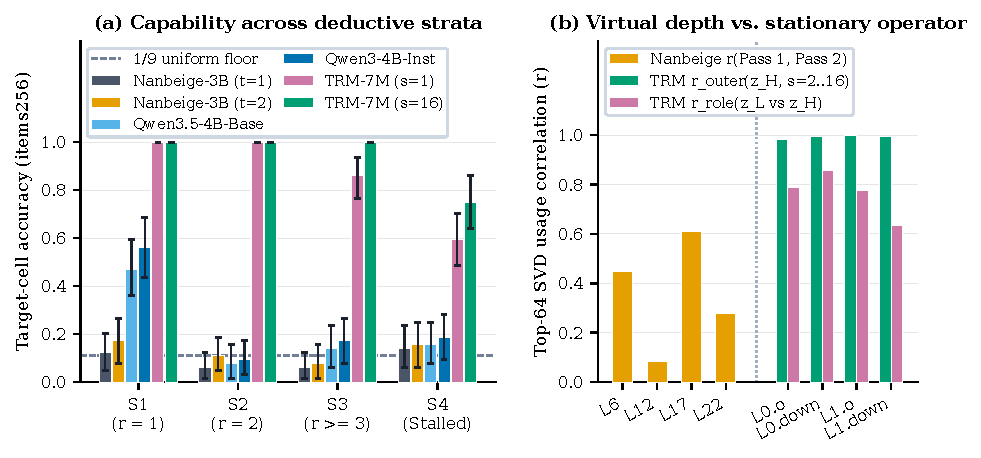
\includegraphics[width=\linewidth]{figures/fig1_virtual_depth_triangulation.pdf}
\caption{\textbf{Regime I vs.\ Regime III on deductively stratified $9\times 9$ Sudoku (\texttt{LOOPSCOPE-02}).} \textbf{(a)} Target-cell accuracy on \texttt{items256} ($n=64$/stratum; 2,000-resample bootstrap 95\% CIs). \texttt{Qwen} models beat \texttt{Nanbeige} strictly on \texttt{S1} ($r=1$), while all three 3B--4B LMs sit near the $1/9 \approx 0.111$ floor on \texttt{S2--S4}; the 7M \texttt{TRM} reaches $1.000$ on \texttt{S1--S3} and $0.750$ target-cell ($0.547$ exact board) on round-0 stalled \texttt{S4}. \textbf{(b)} Top-64 SVD input-usage correlations $r$: \texttt{Nanbeige} multiplexes nonlinear MLP inputs across passes ($\bar{r}=0.355$, $r=0.085$ at \texttt{L12}), whereas \texttt{TRM} iterates a stationary outer operator ($\bar{r}_{\mathrm{outer}}=0.992$) while splitting inner $z_L$ vs.\ $z_H$ calls ($\bar{r}_{\mathrm{role}}=0.765$).}
\label{fig:triangulation}
\end{figure}

\begin{table}[t]
\centering
\small
\begin{tabularx}{\linewidth}{@{}lcccccc>{\raggedright\arraybackslash}X@{}}
\toprule
Model / Pass setting & Params & Overall & \texttt{S1} ($r{=}1$) & \texttt{S2} ($r{=}2$) & \texttt{S3} ($r{\ge}3$) & \texttt{S4} (Stall) & Loop / operator signature \\
\midrule
\texttt{Nanbeige4.2-3B} ($t=1$) & 3.0B & 0.098 & 0.125 & 0.062 & 0.062 & 0.141 & Half virtual pipeline (22L) \\
\texttt{Nanbeige4.2-3B} ($t=2$, native) & 3.0B & 0.129 & 0.172 & 0.109 & 0.078 & 0.156 & Multiplexed SVD ($\bar{r}=0.355$) \\
\texttt{Nanbeige4.2-3B} ($t=8$, OOD) & 3.0B & 0.090 & 0.047 & 0.156 & 0.062 & 0.094 & Non-contractive ($\|\Delta h\|/\|h\|=0.71$) \\
\texttt{Qwen3.5-4B-Base} (untied) & 4.0B & 0.211 & 0.469 & 0.078 & 0.141 & 0.156 & Advantage strictly on \texttt{S1} ($30/64$) \\
\texttt{Qwen3-4B-Instruct} (SDPA) & 4.0B & 0.254 & 0.562 & 0.094 & 0.172 & 0.188 & Untied 36L pure-SDPA control \\
\midrule
\texttt{TRM-7M} ($s=1$: 21 core calls) & 7.0M & 0.863 & 1.000 & 1.000 & 0.859 & 0.594 & Inner sweep; exact board $= 0.082$ \\
\texttt{TRM-7M} ($s=16$: 336 core calls) & 7.0M & \textbf{0.938} & \textbf{1.000} & \textbf{1.000} & \textbf{1.000} & \textbf{0.750} & Stationary ($\bar{r}=0.992$); board $= \mathbf{0.883}$ \\
\bottomrule
\end{tabularx}
\caption{Stratified $9\times 9$ Sudoku target-cell accuracy on \texttt{items256} ($N=256$, $64$ boards/stratum; uniform chance $= 1/9 \approx 0.111$). Note that \texttt{S4} here denotes boards with \emph{zero singles anywhere at round 0} ($n=64$, where \texttt{TRM} $s=16$ target-cell accuracy is $48/64 = 0.750$ and exact 81-cell board solve is $35/64 = 0.547$), distinct from the broader set of $183$ \texttt{items256} boards where whole-board propagation eventually stalls ($153/183 = 0.836$ exact board solve; Table~\ref{tab:fiber_controls}).}
\label{tab:sudoku_triangulation}
\end{table}

\subsection{SVD Input-Subspace Multiplexing and Reconciling \texttt{L12} Residual Alignment}\label{sec:svd_multiplex}

To quantify whether shared matrices execute the same linear sub-operations across passes, let $W_l = \sum_{j} \sigma_{l,j} u_{l,j} v_{l,j}^\top$ be the exact SVD of a shared projection matrix (\texttt{mlp.down\_proj} in \texttt{Nanbeige}; \texttt{o\_proj} and \texttt{down\_proj} in \texttt{TRM}), and define the invocation-$p$ rank-one input-usage profile over top $K=64$ singular directions:
\begin{equation}
  u_{l,p}(j) \;=\; \sigma_{l,j}\,\mathbb{E}_{x \in \mathcal{D}}\bigl[\,|\langle x_{l,p},\, v_{l,j}\rangle|\,\bigr],
  \qquad
  r_l(p,q) \;=\; \operatorname{corr}_{j=1\dots 64}\!\bigl(u_{l,p}(j),\, u_{l,q}(j)\bigr),
  \label{eq:svd_r}
\end{equation}
with $\bar{r}$ denoting the arithmetic mean of $r_l(p,q)$ across audited matrices $l$ (and across outer step pairs $2\le p < q \le 16$ for $\bar{r}_{\mathrm{outer}}$). Across \texttt{Nanbeige} physical layers \texttt{(L6, L12, L17, L22)}, cross-pass correlation averages $\bar{r} = 0.355$ ($r_{\texttt{L6}}=0.448$, $r_{\texttt{L12}}=0.085$, $r_{\texttt{L17}}=0.610$, $r_{\texttt{L22}}=0.277$; Figure~\ref{fig:triangulation}b).

At first glance, near-zero SVD input correlation at \texttt{L12} ($r=0.085$) appears to conflict with high \texttt{L12} residual-stream cosine similarity ($0.799$--$0.869$). The two measurements probe different sites around a nonlinear gate: residual state $h_{12}^{(p)} = h_0^{(p)} + \sum_{\ell \le 12}\Delta_\ell^{(p)}$ is dominated by the shared skip-connection sum accumulated over earlier layers, whereas $x_{\texttt{L12},p}$ entering \texttt{mlp.down\_proj} is the post-\texttt{RMSNorm} \emph{SwiGLU intermediate activation} $\operatorname{SiLU}(W_{\mathrm{gate}}\tilde{h}_{12}^{(p)}) \odot (W_{\mathrm{up}}\tilde{h}_{12}^{(p)})$ in $\mathbb{R}^{d_{\mathrm{ff}}}$. Moderate pass differences in $\tilde{h}_{12}^{(p)}$ switch which multiplicative SwiGLU gates open, routing Pass 1 and Pass 2 into nearly uncorrelated singular input subspaces of \texttt{mlp.down\_proj} even while the ambient residual stream remains macroscopically aligned.

\section{Separating Dynamical Fragility from Component Specificity}\label{sec:fragility}

\subsection{The \texttt{HUG-CAL-02} Rotation Null on \texttt{Huginn-0125}}

On 3-shot variable-binding chains, the 3.5B looped model \texttt{Huginn-0125} \cite{geiping2025huginn} (2-layer prelude, 4-layer tied core with learned adapter input re-injection at every step, 2-layer coda; trained from random Gaussian latent initializations using gradient-free warmup iterations followed by \emph{truncated backpropagation through only the final $k=8$ steps}, and evaluated here at $r=16$) achieves $0.76$ accuracy at 1 hop and $0.47$ at 2 hops ($0.25$--$0.33$ floor at $3$--$6$ hops). Deleting top-16 SVD triplets of core \texttt{mlp.proj} in iterations $1$--$8$ cost $0.00$ nats versus $-0.77$ nats in iterations $13$--$16$. Yet in registered \textbf{Silico Experiment \#3} (\texttt{HUG-CAL-02} \cite{dugan2026hugcal}; 240 clean-correct 2-hop programs $\times$ 3 noise seeds, 8 frozen factors across \texttt{core0--core3}, 4 random orthogonal input-read rotations per factor matched to exact per-iteration projection RMS while fixing write vector $u$), \textbf{factor specialization disappeared}: \texttt{core3 f1} in iterations $9$--$16$ cost $-0.366$ nats raw versus $-0.368$ nats under matched rotation ($+0.0007$ nats net; all 8 factors within $\pm 0.0065$ nats; Figure~\ref{fig:fragility}a). Early ablations are masked by downstream attractor repair; late ablations leave no repair steps before readout.

\begin{figure}[t]
\centering
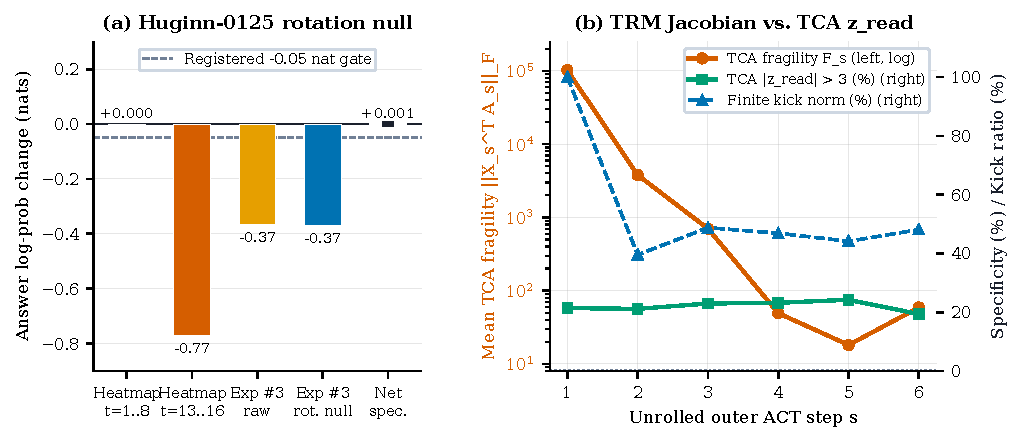
\includegraphics[width=\linewidth]{figures/fig2_fragility_vs_specificity_tca.pdf}
\caption{\textbf{Dynamical fragility vs.\ directional specificity.} \textbf{(a)} Registered \texttt{HUG-CAL-02} (\texttt{Huginn-0125}, $r=16$): late-window SVD ablation loss ($-0.366$ nats) is matched within $\pm 0.0065$ nats by RMS-matched orthogonal read rotations ($-0.368$ nats). \textbf{(b)} Unrolled 6-step \texttt{TCA} on Sudoku \texttt{TRM} (126 core calls; 105 calls between $s=1$ and $s=6$ commits): detached-ACT tangent Jacobians inflate $F_1/F_6 = 1{,}808.4$ while finite $0.25\cdot\mathrm{RMS}$ kicks contract to $30.3\%$; \texttt{TCA}'s rotation $z$-score cancels $\|A_s\|$, isolating a flat $22.04\%$ read-specific circuit.}
\label{fig:fragility}
\end{figure}

\subsection{Transported Component Attribution (\texttt{TCA}) and the Detached-ACT Lyapunov Contrast}

To avoid running multi-pass empirical rotation sweeps per factor, \textbf{Transported Component Attribution (\texttt{TCA})} (\texttt{LOOPSCOPE-01} \cite{dugan2026loopscope01}) computes both fragility and exact Haar-rotation specificity in \emph{one forward and backward pass}. For input activations $X_{l,t} \in \mathbb{R}^{P \times d_{\mathrm{in}}}$ to $W_l \in \mathbb{R}^{d_{\mathrm{out}} \times d_{\mathrm{in}}}$ at call $t$ and backpropagated readout gradient $A_{l,t} = \partial y / \partial (X_{l,t} W_l^\top) \in \mathbb{R}^{P \times d_{\mathrm{out}}}$, deleting rank-one term $\sigma u v^\top$ has first-order effect $\Delta_{l,t}(u,v) = -\sigma v^\top (X_{l,t}^\top A_{l,t}) u$, pure \textbf{dynamical fragility} $F_{l,t} = \|X_{l,t}^\top A_{l,t}\|_F$, and exact Haar-orthogonal read/write $z$-scores:
\begin{equation}
  z_{\mathrm{read}}(u,v) \;=\; \frac{\Delta_{l,t}(u,v)}{\sigma \|v\|_2 \, \|X_{l,t}^\top A_{l,t} u\|_2 / \sqrt{d_{\mathrm{in}}}},
  \qquad
  z_{\mathrm{write}}(u,v) \;=\; \frac{\Delta_{l,t}(u,v)}{\sigma \|u\|_2 \, \|A_{l,t}^\top X_{l,t} v\|_2 / \sqrt{d_{\mathrm{out}}}}.
  \label{eq:tca_z}
\end{equation}

We validated \texttt{TCA} in two complementary regimes. First, on \texttt{Huginn-0125} (\texttt{LOOPSCOPE-01} \texttt{Q1}--\texttt{Q2}), summing $\Delta_{l,t}$ across \textbf{480 measured multi-iteration ablation conditions}—$\bigl(16 \text{ top SVD} + 8 \text{ random directions}\bigr) \times 4 \text{ core layers} \times 5 \text{ iteration windows}$—achieved Spearman $\rho = 0.75$ and $93\%$ sign agreement for $|\text{measured}| \ge 0.05$ nats, validating first-order $\Delta_{l,t}$ transport on a model where true specificity is null ($|z_{\mathrm{read}}| \le 1.8$ on top \texttt{core3} factors; $8.6\%$ of $4{,}096$ cells above $3\sigma$). Second, directional specificity $z_{\mathrm{read}}$ itself was validated against exact central finite differences ($r > 0.9999$), 2,000-sample Monte Carlo Haar rotations, and ground-truth edge-slot circuits in \texttt{LoopedChase}.

In \texttt{LOOPSCOPE-02}, each outer ACT step of the 2-layer Sudoku \texttt{TRM} executes $3$ $H$-cycles $\times (6 \text{ inner } z_L \text{ calls} + 1 \text{ commit } z_H \text{ call}) = \mathbf{21}$ \texttt{L\_level} core calls ($42$ transformer layers), totaling $16 \times 21 = 336$ core calls at $s=16$. Unrolling 6 outer steps in float32 executes $6 \times 21 = 126$ core calls, with $\mathbf{5 \times 21 = 105}$ intermediate core calls separating the $s=1$ commit call (\texttt{\#21}) from the $s=6$ commit call (\texttt{\#126}). This prospectively falsified pre-registered gate \texttt{P4} ($\bar{F}_1/\bar{F}_6 \le 0.25$) in the opposite direction, revealing an observational \textbf{Detached-ACT vs.\ BPTT Lyapunov Contrast} across our model suite (Table~\ref{tab:tca_summary}; note this is a cross-architecture comparison rather than a controlled retraining of \texttt{TRM} under 336-call BPTT):
\begin{itemize}
  \item \textbf{Multi-step and truncated BPTT loopers} differentiate across multiple consecutive recurrent steps during training—either end-to-end (\texttt{Lean S-loop}, extrapolating \texttt{LoopedChase}) or via truncated BPTT over the final $k=8$ recurrent steps after gradient-free warmup from random Gaussian starts (\texttt{Huginn-0125} \cite{geiping2025huginn})—penalizing positive multi-step tangent Lyapunov exponents and yielding $F_1 / F_{\mathrm{late}} < 1$ ($0.43$ on \texttt{Huginn}; $0.007$ on \texttt{Lean} log-$p$).
  \item \textbf{1-step detached ACT (\texttt{HRM}/\texttt{TRM} \cite{wang2025hrm,jolicoeur2025trm})} inherits \texttt{HRM}'s 1-step gradient approximation: \texttt{TRM} detaches $(z_H, z_L)$ between outer steps and runs the first $2$ of $3$ $H$-cycles ($14$ of $21$ core calls/step) under \texttt{torch.no\_grad()}, backpropagating through only a single 7-call $H$-cycle per outer step. Nonlinear \texttt{Post-RMSNorm} dynamics contract \emph{finite} $0.25\cdot\mathrm{RMS}$ kicks monotonically ($1.000 \to 0.303$ by $s=16$), yet unpenalized 105-call tangent Jacobians expand at $\approx 1.074\times$ per core call ($1.074^{105} \approx 1.8\times 10^3$), giving mean $\bar{F}_1/\bar{F}_6 = \mathbf{1{,}808.4}$ (and a single-matrix maximum swing of $6{,}400\times$--$7{,}048\times$ on \texttt{L0.down\_proj}: $148{,}723$ at $s=1$ vs.\ $21.1$ at $s=5$).
\end{itemize}
While Kaissis et al.\ \cite{kaissis2026sdi} formulated \texttt{SDI} to decompose TracIn training-data influence inside BPTT-trained loopers (we did not run TracIn), our Jacobian result provides an analytical transfer caution: applying unnormalized $\sum \delta_s \otimes a_s$ step outer products to detached-ACT checkpoints would weight step 1 over step 6 by three orders of magnitude from tangent expansion alone. Because $\|A_s\|$ cancels identically in Equation~\eqref{eq:tca_z}, \texttt{TCA} recovers a step-invariant $\mathbf{22.04\%}$ share of $|z_{\mathrm{read}}| > 3$ components ($81.6\times$ the $0.27\%$ Gaussian null) and $12.37\%$ write-specific components.

\begin{table}[t]
\centering
\small
\begin{tabularx}{\linewidth}{@{}llcccc>{\raggedright\arraybackslash}X@{}}
\toprule
Model & Training gradient & Re-inject? & $F_1 / F_{\mathrm{late}}$ & $|z_{\mathrm{read}}|{>}3$ & Kick & Mechanistic regime \\
\midrule
\texttt{Nanbeige4.2-3B} & 2-pass BPTT & No & $0.42$--$2.00$ & $0.9\%$--$8.4\%$ & $6.90\times$ & Virtual depth; non-contractive \\
\texttt{Qwen3.5-4B-Base} & Untied 36L & --- & --- & $0.2\%$--$19.9\%$ & --- & Specific at final \texttt{L32} ($19.9\%$) \\
\texttt{Huginn-0125} ($r{=}16$) & Trunc.\ BPTT ($k{=}8$) & Yes (adapter) & $0.43$ & $8.6\%$ & Contr. & Random-init warmup; \texttt{HUG-CAL-02} null \\
\LoopT\ ($T{=}8$, \texttt{RMP}) & 8-step BPTT & No (prompt) & $< 1$ & Sparse & Contr. & Closed-loop SAE/DAS transfer \\
\texttt{Lean S-loop} ($T{=}32$) & Multi-step BPTT & Yes & $0.007$ & $5\%$--$11\%$ & Contr. & Attractor masking ($150\times$) \\
\texttt{LoopedChase} ($24$ arms) & 8-step BPTT & Yes ($\mathrm{LN}{+}e$) & $0.08$--$0.36$ & Edge slots & Contr. & Head-readable ($\lambda{\ge}0.1$: $1.00$) \\
\texttt{TRM-7M} (Sudoku) & Detached ACT & Yes ($z_H{+}x$) & $\mathbf{1{,}808.4}$ & $\mathbf{22.04\%}$ & $\mathbf{0.303\times}$ & Basin-contractive, tangent-exp. \\
\bottomrule
\end{tabularx}
\caption{Summary of training regime, prompt/input re-injection \cite{olszowiec2026monitoring}, \texttt{TCA} fragility ratio, read specificity share ($3\sigma$ Gaussian null $= 0.27\%$), and macroscopic kick response across all studied model families.}
\label{tab:tca_summary}
\end{table}

\section{Regime II: Closed-Loop Dictionaries, Mediated Variables, and Head-Readable Staircases}\label{sec:regime2}

\subsection{Matched Tied vs.\ Untied Training and Closed-Loop Surrogates (\texttt{RMP})}

Consistent with Sesodia et al.\ \cite{sesodia2026inside}, training matched $d=128$ transformers across four reference-trace tasks in \texttt{RMP} \cite{dugan2026rmp} showed \LoopT\ (1 block $\times 8$ loops, 0.46M params, no explicit re-injection beyond non-cursor prompt tokens) passing the $G_0 = 0.98$ \texttt{EM} gate in $6/6$ seeds versus $3/6$ in untied \FFU\ (8 blocks, 1.84M params). Closed-loop insertion of a single shared TopK \texttt{SAE} after all 8 visits retained $0.923, 0.910, 0.900$ of clean deep \texttt{EM} in \LoopT\ seeds 1--3 versus $0.688$ in untied \FFU\ seed 3 (below matched PCA $0.796$ and equal-norm isotropic Gaussian noise $0.778$); shared MLP-only transcoders \cite{dunefsky2024transcoders} with live attention retained $0.940$--$0.996$ across 9 models at $3.5\times$ lower active coding rate ($342$ vs.\ $1{,}213$ bits). While answer-token probes decoded $\cur(s)$ ($0.76$--$1.00$) without causal patch effect ($\IIA \le 0.22$) \cite{geiger2024das,makelov2024illusion}, patching the query+answer block transferred early hops ($\IIA = 0.67$--$1.00$, start-copy $\le 4.5\%$), and $\le 32$ shared-dictionary features mediated $\cur(s)$ on $1{,}000$ collision-free pairs in $4/5$ tied seeds ($0.605$--$1.000$) vs.\ $0/2$ untied ($0.277, 0.386$).

\subsection{Monitorability Frontier and Contrast Projection (\texttt{LOOPSCOPE-01})}

On \texttt{Lean-CGRT} (\texttt{Q3}, \texttt{Q6}), \texttt{S-loop} scaled certified proof rate from $48.6\%$ ($T=8$) to $65.0\%$ ($T=32$) while decoding final tactics via its unmodified head at $94\%$--$99\%$ by $T/2$. Across 24 depth-8 \texttt{LoopedChase} models ($12$ \texttt{Q4} discovery + $12$ \texttt{Q5} prospective, $\lambda \in \{0, 0.01, 0.1, 1\}$), $\lambda \ge 0.1$ achieved $1.00$ depth-9--16 extrapolation and $1.00$ head readability. Notice how this refines Olszowiec et al.\ \cite{olszowiec2026monitoring}: every \texttt{LoopedChase} arm re-injects prompt embeddings via $h \leftarrow \operatorname{LN}(h) + e$, yet $5/9$ $\lambda=0$ arms still fail OOD extrapolation via deadline schedule desynchronization, whereas \LoopT\ succeeds without explicit re-injection by preserving prompt tokens in context. Thus input re-injection stabilizes deep state carry without alone enforcing time-invariant operator simulation; training-depth own-head belief commutation error $\hat{E}$ (\texttt{Q11}) diagnoses true operator simulation at $\mathbf{AUC = 0.992}$ (Figure~\ref{fig:compactification}a; corroborated by \texttt{SEM-ECHO-01}, $\rho=0.92$).

\begin{figure}[t]
\centering
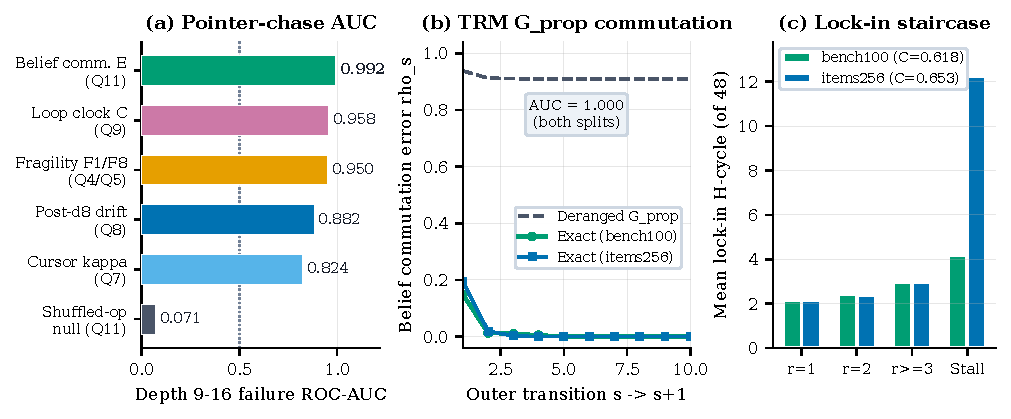
\includegraphics[width=\linewidth]{figures/fig3_compactification_staircase.pdf}
\caption{\textbf{Compactification commutation laws.} \textbf{(a)} ROC-AUC predicting depth-9--16 failure across 24 \texttt{LoopedChase} arms (\texttt{Q11} belief commutation $\hat{E}$ reaches $\mathrm{AUC}=0.992$). \textbf{(b)} Sudoku \texttt{TRM} visible beliefs commute with exact $\Gprop$ ($\rho_{\mathrm{clean}} \to 0.000$ by $s=4$; $\mathrm{AUC}=1.000$ vs.\ deranged clues on both splits). \textbf{(c)} Mean lock-in $H$-cycle (of 48) follows $r=1 < r=2 < r\ge 3 < \text{stalled}$ ($C_{\mathrm{stair}} = 0.653$ vs.\ $0.495$ null on \texttt{items256}).}
\label{fig:compactification}
\end{figure}

\paragraph{The Markovian contrast control and the readout blind spot.} To test whether erasing head-orthogonal state harms a Regime II model, we projected the 256-d carried cursor $h_{t,\mathrm{cursor}}$ of all 24 \texttt{LoopedChase} checkpoints onto the 16-d effective row space $\Phead$ of $\texttt{head}\circ\texttt{ln\_f}$ (removing $240/256$ dimensions after every loop $1\dots 16$; Figure~\ref{fig:dark_fiber}b). At $\lambda = 0.1$, \textbf{all $3/3$ seeds retained $1.000$ depth-1--8 and $1.000$ held-out depth-9--16 accuracy} under raw $\Phead$ projection, LayerNorm-moment-preserved projection, donor-swapped orthogonal fiber, and step-1 frozen fiber (and $8/9$ extrapolating $\lambda \in \{0.01, 0.1\}$ seeds across \texttt{Q4}+\texttt{Q5} retained $0.982$--$1.000$). At $\lambda = 1.0$, however, seed 1 collapsed to $0.129$ under cursor $\Phead$ projection even with LayerNorm statistics restored (mean $0.710$), and our \texttt{Resume} audit in Section~\ref{sec:loopscope03} reveals that \emph{two} of the three $\lambda=1.0$ seeds rely on trajectory-dependent hidden state ($\mathrm{Price}(R_4) = +3.06$ and $+5.46$ loops in seeds 1--2, vs.\ $0.00$ across all $3/3$ $\lambda=0.1$ seeds). This directly instantiates Sharma and Vu's \cite{sharma2026dense} \textbf{readout blind spot (visibility--activity mismatch)}: dense per-loop cross-entropy supervises only readout-visible coordinates ($\Phead$) at each step without penalizing computation routed through $\ker(\texttt{head}\circ\texttt{ln\_f})$ across steps, so maximal intermediate supervision ($\lambda=1.0$) does \emph{not} enforce head-only reasoning and here leaves more dark state than moderate $\lambda=0.1$. Projecting non-cursor edge-table tokens (\texttt{all\_tokens\_fiber\_erased}) collapsed accuracy to $0.177$ because $\texttt{head}$ reads node IDs rather than $(u,v)$ edge bindings. Thus Markovian chain propagation \emph{admits} zero-dark-memory solutions ($3/3$ seeds at $\lambda=0.1$) without dense readout supervision guaranteeing them ($1/3$ pure head-readable seeds at $\lambda=1.0$).

\section{Regime III: Stationary Attractor Search and Head-Orthogonal Controls}\label{sec:regime3}

We now turn to the frozen 7M-parameter, 2-layer Attention-\texttt{TRM} (\texttt{gaoxin492/\allowbreak TinyRecursiveModels-\allowbreak Sudoku-\allowbreak Extreme-\allowbreak att}, \texttt{step\_21700}, $d=512$, 16 outer steps $\times$ 21 core calls $= 336$ passes; replicated on independent checkpoint \texttt{yagizdevre/\allowbreak trm-\allowbreak sudoku-\allowbreak extreme-\allowbreak att} \cite{jolicoeur2025trm}) across \texttt{items256} ($73$ whole-board $\Gprop$-solvable [\texttt{WB-Prop}], $183$ eventually stalling [\texttt{WB-Stall}]) and \texttt{bench100} ($49$ \texttt{WB-Prop}, $51$ \texttt{WB-Stall}). Architectural credit for the dual-state design and backtracking hypothesis belongs to Wang et al.\ \cite{wang2025hrm} (\texttt{HRM}) and Jolicoeur-Martineau \cite{jolicoeur2025trm} (\texttt{TRM}): \texttt{HRM} introduced coupled high- and low-level states $(z_H, z_L)$ trained under 1-step equilibrium gradients from a fixed initial state, qualitatively observing depth-first-like Sudoku backtracking (\cite{wang2025hrm}, Fig.~7) and higher participation dimensionality in $z_H$ than $z_L$ (\cite{wang2025hrm}, Fig.~8), while \texttt{TRM} collapsed \texttt{HRM} into one shared 2-layer network and interpreted $z_H$ ($y$ in \cite{jolicoeur2025trm}) as the embedded current proposed solution and $z_L$ ($z$ in \cite{jolicoeur2025trm}) as a latent reasoning scratchpad enabling multi-step backtracking. Building on those priors, we test pre-stall $\Gprop$ commutation quantitatively and intervene causally on $(I-\Phead)z_H$ and $z_L$ separately and jointly.

\subsection{Two-Timescale Convergence, Corruption Repair, and \texorpdfstring{$\Gprop$}{G\_prop} Commutation (\texttt{P1}--\texttt{P5})}

As audited in Table~\ref{tab:verdicts}, \texttt{TRM} factors Sudoku across two timescales:
\begin{enumerate}[topsep=3pt,itemsep=2pt]
  \item \textbf{Inner 21-call sweep ($s=1$) vs.\ outer steps $s=2\dots 16$:} Step $s=1$ already reaches $0.863$ target-cell accuracy ($1.000$ on \texttt{S1--S2}) but only $0.082$ ($21/256$) exact full-board solve. Outer steps $2\dots 16$ drive exact board solve to $\mathbf{0.883}$ ($226/256$) on \texttt{items256} and $\mathbf{1.000}$ ($100/100$) on \texttt{bench100} ($\mathbf{0.719}$ [$184/256$] on \texttt{items256} and $\mathbf{0.920}$ [$92/100$] on \texttt{bench100} on the independent \texttt{yagizdevre} replication checkpoint). Corrupting 10 empty cells of $z_H(1)$ with donor states drops $s=1$ exact board solve to $0.000$ ($0/256$) and self-repairs by $s=16$ to $\mathbf{0.887}$ ($227/256$, $p=9.27\times 10^{-69}$)—exceeding clean $0.883$ ($226/256$) by one board because all $226$ clean-solved boards recover while the step-1 perturbation dislodges one marginally stalled board into the valid basin.
  \item \textbf{Pre-stall $\Gprop$ commutation and post-stall conflict flips:} Visible \texttt{lm\_head} probabilities commute with exact $\Gprop$ on \texttt{WB-Prop} boards ($\rho_s \to 0.000$ by $s=4$, $\mathrm{AUC}=1.000$; Figure~\ref{fig:compactification}b), and lock-in times across all 48 $H$-cycles obey $2.14 < 2.35 < 2.97 < 12.22$ on \texttt{items256} ($C_{\mathrm{stair}}=0.6531$ vs.\ $0.4947$ null; engaging Wu et al.'s \cite{wu2026shared} observation of uneven step progress by tying commit timing directly to deductive round $r(i)$). Past stall, \texttt{TRM} solves $51/51$ ($100\%$) of \texttt{bench100} \texttt{WB-Stall} boards and $153/183$ ($83.6\%$) of \texttt{items256} \texttt{WB-Stall} boards (including $35/64 = 54.7\%$ exact board solve and $48/64 = 75.0\%$ target-cell accuracy on strict round-0 zero-single \texttt{S4\_stalled}), traversing explicit Sudoku unit violations on $98.0\%$--$99.3\%$ of solved stalled boards ($13.90 \to 0.00$ violated units on \texttt{bench100}; Figure~\ref{fig:dark_fiber}a) via $107.8$--$128.0$ non-monotone cell flips.
\end{enumerate}

\begin{table}[t]
\centering
\small
\begin{tabularx}{\linewidth}{@{}ll>{\raggedright\arraybackslash}p{0.31\linewidth}>{\raggedright\arraybackslash}X@{}}
\toprule
Hypothesis & Verdict & Registered threshold behavior & Structural mechanism isolated (with follow-up controls) \\
\midrule
\texttt{P1} Triangulation & Not supported & 3/4 met; single-cell $\Delta_{1\to 16} = +0.074 < 0.25$ & $s{=}1$ (21 core calls) reaches $0.863$ target-cell; $s{=}2..16$ drives full-board exact solve $0.082 \to 0.883$ ($+0.801$) \\
\texttt{P2} Attractor vs.\ VD & Not supported & Repair \& \texttt{NB} drift met; single-cell open drop $0.074 < 0.30$ & 10-cell donor corruption collapses $s{=}1$ board solve to $0.000$ and repairs to $0.887$ ($227/256$); kicks contract $0.303\times$ \\
\texttt{P3} SVD geometry & Weak & \texttt{TRM} $\bar{r}_{\mathrm{outer}}=0.992$, $\bar{r}_{\mathrm{role}}=0.765$; \texttt{NB} $\bar{r}=0.355 \in [0.3, 0.4)$ & \texttt{Nanbeige} SwiGLU multiplexing (\texttt{L12} $0.085$) vs.\ \texttt{TRM} stationary outer operator + inner $z_L/z_H$ role split \\
\texttt{P4} Unrolled \texttt{TCA} & Not supported & Specificity $22.04\% \gg 1.35\%$; $F_1/F_6 = 1{,}808.4 \gg 0.25$ & Detached-ACT tangent expansion (105 calls between $s{=}1,6$ commits) coexists with $0.303\times$ basin contraction \\
\texttt{P5} Compactification & \textbf{Supported} & \textbf{5/5 sub-criteria met} ($p \le 2\times 10^{-28}$) & $\Gprop$ commutation ($\mathrm{AUC}=1.000$); manifold + replication controls separate off-manifold norm loss from stalled-search transition dynamics \\
\bottomrule
\end{tabularx}
\caption{Pre-registered \texttt{LOOPSCOPE-02} verdicts and calibrated mechanistic findings.}
\label{tab:verdicts}
\end{table}

\subsection{Dissecting Head-Orthogonal Projection: Norm Collapse, Checkpoint Replication, and History Probes}\label{sec:fiber_controls}

Because \texttt{TRM}'s vocabulary has size $11$, $\texttt{lm\_head.weight} \in \mathbb{R}^{11 \times 512}$ has exact rank $11$, defining an 11-d readout row space $\Phead$ and a \textbf{501-dimensional head-orthogonal fiber} $(I - \Phead)\mathbb{R}^{512} = \ker(\texttt{lm\_head})$. In pre-registered test \texttt{P5}, resetting $z_L \leftarrow L_{\mathrm{init}}$ between outer steps preserved $99/100$ ($0.990$) on \texttt{bench100} and $213/256$ ($0.832$) on \texttt{items256}, whereas raw \texttt{fiber\_erased} ($z_H^{\mathrm{board}} \leftarrow z_H^{\mathrm{board}}\Phead + H_{\mathrm{init}}(I-\Phead)$ plus \texttt{reset\_zL}) collapsed solve to $0.070$ ($7/100$) on \texttt{bench100} ($0/100$ on \texttt{yagizdevre} replication) and $0.066$ ($17/256$; $0/256$ replication) on \texttt{items256}. Auditing batch size ($\mathrm{bsz}\in\{1,50,64,100\}$), arithmetic precision (\texttt{bfloat16} vs.\ \texttt{float32}), and projector SVD precision explains why raw \texttt{fiber\_erased} scored $7/100$ in \texttt{P5} (\texttt{bsz}=50, GPU \texttt{float32} SVD) versus $5/100$ in our control runner (\texttt{bsz}=64, CPU \texttt{float64} SVD): at \texttt{bsz}=64 in \texttt{bfloat16}, GPU \texttt{float32} vs.\ CPU \texttt{float64} SVD accounts for $7/100$ vs.\ $5/100$, while \texttt{bfloat16} cuBLAS/SDPA batch-tile non-associativity across 336 recursive passes shifts borderline off-manifold trajectories between $4/100$ and $7/100$ across batch sizes ($6, 4, 5, 7$ at $\mathrm{bsz}=1, 50, 64, 100$ under \texttt{float64} SVD; $3$--$4/100$ in \texttt{float32}). By contrast, on-manifold \texttt{clean} and \texttt{bfloat16} \texttt{fiber\_norm\_restored} are deterministically $\mathbf{100/100}$ across all four batch sizes.

Inspecting raw \texttt{fiber\_erased} \emph{by stratum} exposes why off-manifold projection was confounded (Table~\ref{tab:fiber_controls}): raw \texttt{fiber\_erased} (and \texttt{zH\_fiber\_only\_erased}, which keeps $z_L$ live: $0.060$ on \texttt{bench100}, $0.070$ on \texttt{items256}) destroys \textbf{propagation-solvable boards too} ($5/49$ on \texttt{bench100}; $17/73 = 0.233$ primary and $0/73$ replication on \texttt{items256}, even while single target cells in \texttt{S1}/\texttt{S2} stay at $0.984/0.969$). Whereas \texttt{LoopedChase} re-normalizes $h \leftarrow \operatorname{LN}(h) + e$ before input addition, \texttt{TRM}'s \texttt{run\_l\_level} feeds $z_H + x_{\mathrm{emb}}$ \emph{without normalization}: both radial norm $\|z_H\|_2$ and the 501-d subspace $\ker(\texttt{lm\_head})$ sit inside Sharma and Vu's \cite{sharma2026dense} readout blind spot (unconstrained by single-step token cross-entropy yet active in the next block call), so zeroing $501/512$ coordinates collapses $\|z_H\|_2$ against $\sqrt{512}$-scaled $x_{\mathrm{emb}}$ and strips the trained \texttt{Post-RMSNorm} carrier offset.

\begin{figure}[t]
\centering
\includegraphics[width=\linewidth]{figures/fig4_dark_fiber_ablation.pdf}
\caption{\textbf{Conflict repair, manifold controls, and two-checkpoint PCA dose-response.} \textbf{(a)} On \texttt{bench100}, \texttt{TRM} solves $49/49$ \texttt{WB-Prop} and $51/51$ \texttt{WB-Stall} boards, driving violated Sudoku units from $13.9 \to 0.0$. \textbf{(b)} Separating off-manifold norm loss from stalled-search fiber sensitivity: raw $\Phead$ fails on \texttt{TRM Prop} ($0.233$) via unnormalized $\|z_H\|_2$ shrinkage, whereas restoring cell L2 norm or grafting donor fibers preserves $1.000$ on both \texttt{LoopedChase} ($\lambda=0.1$) and primary \texttt{TRM Prop} ($73/73$), leaving a $-8.7$~pp drop on primary \texttt{WB-Stall} ($0.836 \to 0.749$, $p=8.6\times 10^{-4}$) and $-15.6$~pp on \texttt{S4} ($0.547 \to 0.391$; $0.328$ under step-1 freeze). \textbf{(c)} Top-$k$ orthogonal PCA dose curves on \texttt{items256} (fitted strictly on \texttt{train.csv}): primary \texttt{gaoxin492} recovers by $k=64$ ($0.831$ vs.\ $0.836$, $p=1.00$), whereas replication \texttt{yagizdevre} (\texttt{Repl.\ Stall}, dashed) dips non-monotonically at intermediate $k \in [4, 64]$ ($0.519$ at $k=16$) before recovering at $k \ge 128$.}
\label{fig:dark_fiber}
\end{figure}

\begin{table}[t]
\centering
\scriptsize
\setlength{\tabcolsep}{2.2pt}
\resizebox{\linewidth}{!}{%
\begin{tabular}{@{}lcccccccccc@{}}
\toprule
Inter-step condition ($s \ge 1$) & \multicolumn{2}{c}{\texttt{bench100} Prim.\ (Repl.)} & \multicolumn{2}{c}{\texttt{items256} WB Prim.\ (Repl.)} & \multicolumn{3}{c}{\texttt{S1--S3} Prim.} & \multicolumn{2}{c}{\texttt{S4} (64) Board [Cell]} & $p_{\mathrm{McNemar}}$ \texttt{WB-Stall} \\
\cmidrule(lr){2-3}\cmidrule(lr){4-5}\cmidrule(lr){6-8}\cmidrule(lr){9-10}
 & Prop (49) & Stall (51) & Prop (73) & Stall (183) & \texttt{S1} & \texttt{S2} & \texttt{S3} & Prim. & Repl. & Prim.\ / Repl. \\
\midrule
Clean $s=16$ (full 512-d) & 1.00 (0.92) & 1.00 (0.92) & \textbf{1.000} (\textbf{0.877}) & \textbf{0.836} (\textbf{0.656}) & 1.00 & 0.98 & 1.00 & \textbf{0.55} [0.75] & \textbf{0.41} [0.70] & --- / --- \\
\texttt{reset\_zL} ($z_L \leftarrow L_{\mathrm{init}}$) & 1.00 (0.92) & 0.98 (0.84) & 1.000 (0.890) & 0.765 (0.628) & 0.97 & 0.95 & 0.95 & 0.45 [0.72] & 0.38 [0.75] & $2.4\text{e-}4$ / $0.54$ \\
Raw \texttt{fiber\_erased} (\texttt{P5}) & 0.10 (0.00) & 0.00 (0.00) & 0.233 (0.000) & 0.000 (0.000) & 0.16 & 0.02 & 0.09 & 0.00 [0.50] & 0.00 [0.39] & $1.8\text{e-}46$ / $1.5\text{e-}36$ \\
\texttt{zH\_fiber\_only\_erased} & 0.12 (0.00) & 0.00 (0.00) & 0.247 (0.000) & 0.000 (0.000) & 0.16 & 0.06 & 0.06 & 0.00 [0.56] & 0.00 [0.48] & $1.8\text{e-}46$ / $1.5\text{e-}36$ \\
\midrule
\texttt{fiber\_norm\_restored} ($k{=}0$) & 1.00 (0.98) & 1.00 (0.88) & \textbf{1.000} (\textbf{0.973}) & \textbf{0.749} (0.590) & 0.97 & 0.97 & 0.95 & \textbf{0.39} [0.67] & \textbf{0.28} [0.64] & $8.6\text{e-}4$ / $0.14$ \\
\texttt{fiber\_train\_mean\_filled} & 1.00 (0.96) & 1.00 (0.96) & \textbf{1.000} (\textbf{0.918}) & \textbf{0.760} (0.639) & 0.98 & 0.95 & 0.97 & \textbf{0.41} [0.73] & \textbf{0.28} [0.64] & $4.3\text{e-}3$ / $0.78$ \\
\texttt{fiber\_donor\_swapped} & 1.00 (0.92) & 1.00 (0.92) & \textbf{1.000} (\textbf{0.904}) & \textbf{0.754} (\textbf{0.557}) & 0.97 & 0.95 & 0.98 & \textbf{0.39} [0.69] & \textbf{0.19} [0.58] & $1.5\text{e-}3$ / $0.022$ \\
\texttt{fiber\_step1\_frozen} & 0.98 (0.98) & 0.92 (0.94) & 0.973 (\textbf{0.932}) & \textbf{0.678} (\textbf{0.486}) & 0.94 & 0.91 & 0.88 & \textbf{0.33} [0.66] & \textbf{0.27} [0.64] & $1.1\text{e-}6$ / $3.7\text{e-}4$ \\
\midrule
Orth.\ PCA $k=0$ ($0\%$ var) & 1.00 (0.98) & 1.00 (0.90) & \textbf{1.000} (\textbf{0.932}) & \textbf{0.760} (0.579) & 0.97 & 0.95 & 0.97 & 0.42 [0.69] & 0.31 [0.67] & $4.3\text{e-}3$ / $0.076$ \\
Orth.\ PCA $k=16$ ($50\%$ var) & 1.00 (0.82) & 1.00 (0.90) & 0.986 (0.904) & 0.798 (\textbf{0.519}) & 0.97 & 0.97 & 0.98 & 0.48 [0.77] & 0.28 [0.66] & $0.12$ / $1.6\text{e-}3$ \\
Orth.\ PCA $k=64$ ($87\%$--$90\%$ var) & 1.00 (0.90) & 1.00 (0.78) & \textbf{1.000} (0.877) & \textbf{0.831} (\textbf{0.579}) & 1.00 & 0.94 & 0.98 & \textbf{0.59} [0.83] & 0.33 [0.69] & $1.00$ / $0.044$ \\
Orth.\ PCA $k=128$ ($97\%$--$99\%$ var) & 1.00 (0.88) & 1.00 (0.94) & \textbf{1.000} (0.877) & \textbf{0.825} (\textbf{0.617}) & 1.00 & 0.95 & 0.98 & 0.56 [0.83] & \textbf{0.41} [0.73] & $0.80$ / $0.35$ \\
Orth.\ PCA $k=501$ ($100\%$ var) & 1.00 (0.92) & 1.00 (0.92) & \textbf{1.000} (\textbf{0.877}) & \textbf{0.836} (\textbf{0.656}) & 1.00 & 0.98 & 1.00 & \textbf{0.55} [0.75] & \textbf{0.41} [0.70] & $1.00$ / $1.00$ \\
\bottomrule
\end{tabular}%
}
\caption{Exact 81-cell board solve across both checkpoints—primary \texttt{gaoxin492} and \texttt{yagizdevre} replication in parentheses—on \texttt{bench100} and \texttt{items256} (\texttt{WB-Prop} $n=73$, \texttt{WB-Stall} $n=183$), plus primary \texttt{S1--S3} board solve (target-cell accuracy is $1.00$ on all manifold/PCA rows except \texttt{S3} \texttt{step1\_frozen} $=0.98$; $0.98/0.97/0.83$ on raw \texttt{fiber\_erased}), two-checkpoint \texttt{S4} ($n=64$) board [target-cell] solve, and exact McNemar $p$ vs.\ clean on \texttt{items256} \texttt{WB-Stall}. On \texttt{WB-Prop}, no manifold-preserving control drops below clean on either checkpoint ($p=1.00$ primary; $p \ge 0.065$, all $\ge 66/73$ vs.\ $64/73$ clean on replication).}
\label{tab:fiber_controls}
\end{table}

Pairing manifold-preserving, two-checkpoint PCA, and differential probe controls (all fitted strictly on $200$ \texttt{train.csv} boards with zero test leakage; Tables~\ref{tab:fiber_controls}--\ref{tab:diff_probes}, Figure~\ref{fig:dark_fiber}b--c) yields four calibrated findings:
\begin{enumerate}[topsep=3pt,itemsep=2pt]
  \item \textbf{Propagation-solvable boards show full interventional invariance across both checkpoints:} Rescaling $z_H^{\mathrm{board}}\Phead$ to each cell's pre-projection L2 norm (\texttt{fiber\_norm\_restored}), filling $(I-\Phead)z_H$ with step-$s$ \texttt{train.csv} means (\texttt{fiber\_train\_mean\_filled}), or grafting a donor board's 501-d fiber (\texttt{fiber\_donor\_swapped}) preserves \textbf{$73/73$ ($1.000$, $p=1.00$) on primary \texttt{items256} \texttt{WB-Prop} and $66$--$71/73$ ($0.904$--$0.973$, exceeding clean $64/73 = 0.877$, $p \ge 0.065$) on \texttt{yagizdevre} replication} ($49/49$ primary and $45$--$48/49$ vs.\ $45/49$ clean replication on \texttt{bench100}).
  \item \textbf{Stalled-board dependence separates cross-checkpoint corruption sensitivity from checkpoint-dependent neutral erasure:} Under manifold-preserving $k=0$ interventions, the re-injected $81\times 11$ continuous logit field alone suffices to retain $89.5\%$--$90.8\%$ of primary clean \texttt{items256} \texttt{WB-Stall} solves ($137$--$139$ vs.\ $153/183$) and $88.3\%$--$97.5\%$ of replication solves ($106$--$117$ vs.\ $120/183$; and $51/51$ primary, $45$--$49/51$ vs.\ $47/51$ clean replication on easier \texttt{bench100}). \emph{Actively corrupting} $(I-\Phead)z_H$ with stale conflict state (\texttt{fiber\_step1\_frozen}) or foreign search state (\texttt{fiber\_donor\_swapped}) significantly degrades \texttt{items256} \texttt{WB-Stall} on \textbf{both} checkpoints: $-15.8$~pp ($0.678$, $p=1.1\times 10^{-6}$) and $-8.2$~pp ($0.754$, $p=0.0015$) on primary \texttt{gaoxin492}, and $-16.9$~pp ($0.486$, $89/183$, $p=3.7\times 10^{-4}$) and $-9.8$~pp ($0.557$, $102/183$, $p=0.022$) on \texttt{yagizdevre} (\texttt{S4} drops $0.406 \to 0.188$, $-21.9$~pp, under donor swap). By contrast, \emph{neutral} $k=0$ erasure produces a statistically significant $-7.7$ to $-8.7$~pp stalled deficit on the stronger primary checkpoint ($0.836 \to 0.749$--$0.760$, $p \le 0.0043$; \texttt{S4}: $0.547 \to 0.391$--$0.422$) whereas on weaker \texttt{yagizdevre} overall \texttt{WB-Stall} point drops do not reach significance ($0.656 \to 0.590$ [$p=0.14$], $0.639$ [$p=0.78$], $0.579$ [$p=0.076$], although round-0 stalled \texttt{S4} drops $0.406 \to 0.281$--$0.312$).
  \item \textbf{Variance-ordered PCA is not a monotone causal basis across checkpoints:} On primary \texttt{gaoxin492} \texttt{items256} \texttt{WB-Stall}, retaining top-$k$ train-PCA orthogonal directions recovers clean solve by $k=64$ ($0.760 \to 0.770 \to 0.792 \to 0.798$ at $k=0,4,8,16$, $0.776$ at $k=32$, and $\mathbf{0.831}$ [$152/183$, $p=1.00$] at $k=64$, $86.6\%$ variance). On \texttt{yagizdevre}, however, the PCA dose curve is \textbf{non-monotone}: \texttt{items256} \texttt{WB-Stall} dips below $k=0$ ($0.579$) at intermediate $k \in [4, 64]$ ($0.541$ at $k=4$ [$p=0.0065$], $0.519$ at $k=16$ [$p=0.0016$], $0.579$ at $k=64$ [$p=0.044$]) before recovering only at $k \ge 128$ ($0.617$ at $k=128$ [$p=0.35$], $0.683$ at $k=256$ [$p=0.51$], $0.656$ at $k=501$; $98.8\%$ variance at $k=128$), and \texttt{bench100} \texttt{Stall} likewise dips from $0.902$ ($k=0$) to $0.784$ ($k=64$) before recovering to $0.941$ ($k=128$). Replacing global-mean centering with step-specific \texttt{step\_mean\_orth}$[s]$ narrows but does not eliminate this interference dip on \texttt{yagizdevre} ($0.961 \to 0.804$ at $k=16,64 \to 0.961$ at $k=128$ on \texttt{bench100}; $0.639 \to 0.568$ [$p=0.037$] at $k=8 \to 0.639$ at $k=64$ on \texttt{items256}), showing that truncating correlated orthogonal coordinates at intermediate $k$ can perturb \texttt{yagizdevre} off its search trajectory more than neutral $k=0$ mean fill.
  \item \textbf{Differential search-history probes vs.\ shuffled-label null:} Standard ridge probes confirm $(I-\Phead)z_H(s)$ is linearly decodable rather than probe-opaque ($<1.5\times 10^{-5}$ max logit leak into \texttt{lm\_head}, yet $97.1\%$--$97.8\%$ step-1 candidate masks and $93.5\%$--$100\%$ step-16 digits), but those targets are already available in $\Phead$ plus re-injected clues. To isolate what $(I-\Phead)z_H(s)$ carries \emph{beyond} the visible channel, we trained ridge probes ($\lambda_{\mathrm{ridge}}=25$) strictly on \texttt{train.csv} trajectories across \path{visible_plus_clues} ($[11\text{-d }\Phead,\, 9\text{-d probs},\, 9\text{-d clue mask}]$), \path{orth_top64}, \path{orth_full501}, \path{combined_vis_orth64}, and a \path{shuffled_label_null} baseline (\path{orth_top64} fit to permuted \texttt{train.csv} labels), alongside the parameter-free \textbf{2nd-highest visible \texttt{lm\_head} logit}, evaluated on the $10{,}190$ empty cells of \texttt{items256} \texttt{WB-Stall} across $s \in \{2, 4, 8, 12\}$ (Table~\ref{tab:diff_probes}). The shuffled-label null sits at chance across every step and task ($0.090$--$0.141$ vs.\ $1/9=0.111$ 9-way; $0.445$--$0.564$ vs.\ $0.500$ binary AUC). Crucially, \texttt{TRM} does \emph{not} store a hidden symbolic ``tabu list'' of refuted digits in $\ker(\texttt{lm\_head})$: on newly flipped cells ($\hat{y}_i(s) \neq \hat{y}_i(s-1)$), the runner-up visible \texttt{lm\_head} logit alone recovers $\hat{y}_i(s-1)$ at $\mathbf{61.8\%}$--$\mathbf{82.9\%}$ (and \path{visible_plus_clues} at $51.7\%$--$70.3\%$), outperforming \path{orth_top64} ($28.1\%$--$40.8\%$, though combining channels lifts $s=4$ accuracy from $0.596 \to 0.650$ primary and $0.587 \to 0.631$ replication), and similarly on cells where \texttt{lm\_head} is currently wrong ($50.7\%$--$59.2\%$ visible vs.\ $30.7\%$--$43.9\%$ \path{orth_top64}). Instead, \path{orth_top64} (and \path{orth_full501}) outperforms \path{visible_plus_clues} at \textbf{every audited step $s \in \{2,4,8,12\}$ on both checkpoints} for predicting \textbf{cumulative cell-flip history} ($\mathrm{AUC} = 0.757/0.756$ [\path{full501} $0.809/0.815$] vs.\ $0.629/0.710$ at $s=2$; $0.645$--$0.655$ vs.\ $0.577$--$0.584$ primary and $0.655$--$0.713$ vs.\ $0.598$--$0.611$ replication across $s=4,8,12$) and \textbf{resolved unit-conflict history} on currently conflict-free cells ($0.726/0.736$ [\path{full501} $0.786/0.780$] vs.\ $0.647/0.684$ at $s=2$; \path{combined_vis_orth64} lifts $s=4$ AUC from $0.611 \to 0.660$ primary and $0.611 \to 0.699$ replication). Thus $(I-\Phead)z_H(s)$ encodes \emph{search-transition and conflict-damping history} rather than hidden candidate identities.
\end{enumerate}

\begin{table}[t]
\centering
\scriptsize
\setlength{\tabcolsep}{2.8pt}
\resizebox{\linewidth}{!}{%
\begin{tabular}{@{}lcccccccc@{}}
\toprule
Feature view / baseline & \multicolumn{2}{c}{Cum.\ flip history AUC} & \multicolumn{2}{c}{Resolved conflict AUC} & \multicolumn{2}{c}{Just-refuted digit acc.\ (9-way)} & \multicolumn{2}{c}{True digit ($\hat{y}_s{\neq}y^*$, 9-way)} \\
\cmidrule(lr){2-3}\cmidrule(lr){4-5}\cmidrule(lr){6-7}\cmidrule(lr){8-9}
(\texttt{train.csv}-fit; \texttt{items256} \texttt{WB-Stall}) & $s=2$ & $s=8$ & $s=2$ & $s=8$ & $s=2$ & $s=8$ & $s=2$ & $s=8$ \\
\midrule
\texttt{shuffled\_label\_null} (\texttt{orth\_top64}) & 0.456 / 0.564 & 0.515 / 0.511 & 0.538 / 0.515 & 0.511 / 0.511 & 0.103 / 0.141 & 0.090 / 0.115 & 0.097 / 0.116 & 0.116 / 0.121 \\
Runner-up \texttt{lm\_head} logit (0 params) & --- & --- & --- & --- & \textbf{0.618} / \textbf{0.620} & \textbf{0.768} / \textbf{0.821} & \textbf{0.581} / \textbf{0.592} & \textbf{0.533} / \textbf{0.600} \\
\texttt{visible\_plus\_clues} (29-d) & 0.629 / 0.710 & 0.584 / 0.607 & 0.647 / 0.684 & 0.617 / 0.636 & 0.517 / 0.572 & 0.591 / 0.703 & 0.574 / 0.570 & 0.516 / 0.560 \\
\texttt{orth\_top64} (64-d in $\ker(\texttt{lm\_head})$) & \textbf{0.757} / \textbf{0.756} & \textbf{0.655} / \textbf{0.655} & \textbf{0.726} / \textbf{0.736} & \textbf{0.626} / \textbf{0.668} & 0.408 / 0.336 & 0.281 / 0.322 & 0.376 / 0.439 & 0.307 / 0.386 \\
\texttt{orth\_full501} (501-d in $\ker(\texttt{lm\_head})$) & \textbf{0.809} / \textbf{0.815} & \textbf{0.676} / \textbf{0.683} & \textbf{0.786} / \textbf{0.780} & \textbf{0.653} / \textbf{0.674} & 0.605 / 0.634 & 0.324 / 0.597 & 0.380 / 0.446 & 0.316 / 0.393 \\
\texttt{combined\_vis\_orth64} (93-d) & \textbf{0.766} / \textbf{0.770} & \textbf{0.666} / \textbf{0.663} & \textbf{0.750} / \textbf{0.745} & \textbf{0.658} / \textbf{0.686} & 0.615 / 0.596 & 0.605 / 0.693 & 0.551 / 0.556 & 0.492 / 0.547 \\
\bottomrule
\end{tabular}%
}
\caption{Differential search-history and refuted-digit probes on held-out \texttt{items256} \texttt{WB-Stall} empty cells ($10{,}190$ cells across $183$ stalled boards; entries show Primary \texttt{gaoxin492} / Replication \texttt{yagizdevre}; full $s \in \{2,4,8,12\}$ receipts in \texttt{fiber\_\-replication\_\-and\_\-history\_\-probes.json}). Binary tasks report ROC-AUC (chance $0.500$); 9-way tasks report accuracy (chance $1/9 \approx 0.111$).}
\label{tab:diff_probes}
\end{table}

\section{Three-Ledger Conditional Refill, Covariate-Shift-Free \texttt{Resume}, and Enforced Path Independence (\texttt{LOOPSCOPE-03})}\label{sec:loopscope03}

Fixed-budget state erasure at $s=16$ tests whether an erased channel can be \emph{rebuilt in time} rather than where computation accrued: as Section~\ref{sec:regime3} showed, stationary re-injected \texttt{TRM} loops repair 10-cell corruptions ($0.000 \to 0.887$) and tolerate single-buffer \texttt{reset\_zL} ($0.836 \to 0.765$) when $(I-\Phead)z_H$ remains live. In pre-registered program \texttt{LOOPSCOPE-03} (commit \texttt{b1ec7755}, publicly archived with Stage 1--4 receipts in \url{https://github.com/MoralityLabAI/VPD/tree/main/output/supplements/loopscope03}), we decompose the full carried state $S_t = (z_H(t), z_L(t)) \in \mathbb{R}^{97\times 512} \times \mathbb{R}^{97\times 512}$ into three ledgers:
\begin{equation}
  S_t \;=\; V_t \;\oplus\; C_t \;\oplus\; R_t,
  \qquad
  V_t = z_H^{\mathrm{board}}(t)\Phead,\quad
  C_t = \hat{H}_\theta(x, V_t),\quad
  R_t = H_t - \hat{H}_\theta(x, V_t),
  \label{eq:three_ledgers}
\end{equation}
where $V_t \in \mathbb{R}^{81\times 11}$ is the head-readable logit projection on the 81 board cells, $H_t = \bigl(z_H^{\mathrm{board}}(t)(I-\Phead),\allowbreak\, z_H^{\mathrm{pref}}(t),\allowbreak\, z_L(t)\bigr)$ is the full head-orthogonal and scratchpad hidden state (including the 16 puzzle-prefix tokens), $C_t = \hat{H}_\theta(x, V_t)$ is the \textbf{Conditional Cache} predictable strictly from input clues $x$ and current visible board state $V_t$ (hence reconstructible by an external monitor), and $R_t$ is the \textbf{Trajectory Residual}, combining path-dependent history with any unmodeled refill error. Crucially, replacing $H_t \leftarrow \hat{H}_\theta(x, V_t)$ makes hidden state a deterministic function of $(x, V_t)$, \emph{enforcing path independence} \cite{anil2022path}.

\subsection{Data-Size Scaling, the \texorpdfstring{$z_H \times z_L$}{z\_H x z\_L} Backup Channel, and Closed-Loop Cadence (\texttt{H3.1}--\texttt{H3.3})}

Because \texttt{TRM}'s \texttt{Post-RMSNorm} places each 512-d token on the sphere $\|v\|_2 \approx \sqrt{512} = 22.627$, raw conditional-mean refill shrinks $\|z_{H,i}^\perp\|_2$ via Jensen's inequality and collapses \texttt{WB-Stall} solve ($0.612$ primary, $0.415$ replication), whereas projecting $\hat{z}_{H,i}^\perp$ onto $(I-\Phead)$ and rescaling to $\sqrt{512 - \|V_{t,i}\|_2^2}$ achieves \texttt{float32} \texttt{lm\_head} parity ($2.29\times 10^{-5}$ / $1.53\times 10^{-5}$ max logit diff) and zero orthogonal leak ($1.49\times 10^{-6}$ / $3.76\times 10^{-6}$). Sweeping six architectures \texttt{C1..C6} on \texttt{train.csv[0:900]} saturated in depth on held-out \texttt{val\_100} ($0.844$ \texttt{C5} vs.\ $0.863$ \texttt{C6}; step-indexed \texttt{C5\_stepclock} $= 0.822$), \emph{yet $N=900$ was still data-limited}. Fitting \texttt{C5} (\texttt{2L-512}) across $N_{\mathrm{train}} \in \{100, 300, 900, 2{,}700, 8{,}100\}$ puzzles disjoint from \texttt{val\_100}, \texttt{items256}, and \texttt{bench100} up to canonical digit-relabelling isomorphism raises primary \texttt{val\_100} joint $R^2$ steadily from $0.632 \to 0.754 \to 0.844 \to 0.889 \to \mathbf{0.915}$ ($0.952$ on \texttt{WB-Prop}, $0.912$ on \texttt{WB-Stall}) and raises replication $R^2$ from $0.689$ ($N=900$) to $\mathbf{0.837}$ ($N=8{,}100$; Figure~\ref{fig:three_ledger}a, Table~\ref{tab:loopscope03}).

\begin{figure}[t]
\centering
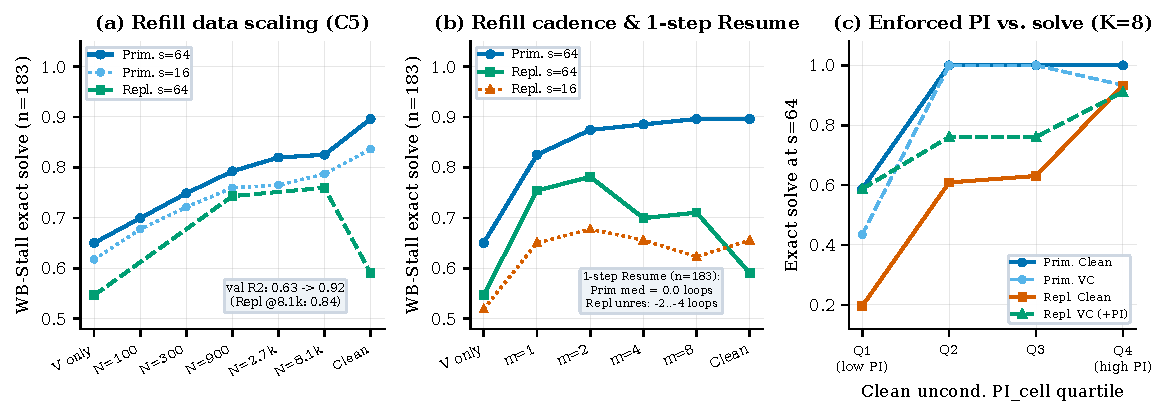
\includegraphics[width=\linewidth]{figures/fig5_three_ledger_pricing.pdf}
\caption{\textbf{Data-scaled conditional refill, periodic cadence vs.\ 1-step \texttt{Resume}, and enforced path independence (\texttt{LOOPSCOPE-03}).} \textbf{(a)} Disjoint training-size scaling ($N=100 \to 8{,}100$) for \texttt{C5\_tf\_2L\_512} on \texttt{items256} \texttt{WB-Stall} ($n=183$): primary held-out $R^2$ rises $0.632 \to 0.915$, narrowing every-step closed-loop loss to $-4.9$~pp ($s=16$) and $-7.1$~pp ($s=64$), while replication ($R^2=0.837$) climbs $+16.9$~pp above clean ($0.590 \to 0.760$ at $s=64$). \textbf{(b)} Closed-loop refill cadence $m \in \{1,2,4,8\}$ ($N=8{,}100$) vs.\ clean: allowing even one unprojected step ($m=2$) restores primary \texttt{WB-Stall} at $s=64$ to $0.874$ ($p=0.289$; $0.896$ at $m=8$, $p=1.00$) and peaks at $0.781$ ($+19.1$~pp, $p=1.2\times 10^{-6}$) on replication; covariate-shift-free 1-step \texttt{Resume} yields $0.0$ median loop delay across unselected primary mutual solvers. \textbf{(c)} Per-board unconditional $\mathrm{PI}_{\mathrm{cell}}(64)$ quartiles ($K=8$ forks, $\sigma=0.35$) vs.\ $s=64$ solve: enforcing path independence via \texttt{VC} rescues low-PI replication boards (\texttt{Q1}: $0.196 \to 0.587$, $+39.1$~pp) while leaving high-PI primary quartiles \texttt{Q2--Q3} at $1.000$.}
\label{fig:three_ledger}
\end{figure}

Evaluating closed-loop and periodic refill across $s \in \{16, 32, 64\}$ (Figure~\ref{fig:three_ledger}a--b, Table~\ref{tab:loopscope03}) establishes four findings:
\begin{enumerate}[topsep=3pt,itemsep=2pt]
  \item \textbf{The $z_H \times z_L$ cross-channel backup (\texttt{H3.1 Supported}):} Single-buffer erasure leaves the partner buffer live to reconstruct search state (\texttt{gaoxin492} \texttt{WB-Stall} at $s=16 \to 64$: $0.749 \to 0.836$ \path{mean_all_zH__live_zL}; $0.792 \to 0.852$ \path{live_zH__mean_zL}). Joint $V$-only erasure of \emph{both} $(I-\Phead)z_H$ (plus prefix) and $z_L$ collapses \texttt{WB-Stall} at $s=16$ to $\mathbf{0.617}$ ($-21.9$~pp, $p=4.6\times 10^{-10}$) on \texttt{gaoxin492} and $\mathbf{0.519}$ ($-13.7$~pp, $p=0.0035$) on \texttt{yagizdevre}, and $4\times$ extra steps ($s=64$) do not rescue it ($0.650$ and $0.546$), trapping $\mathbf{33.3\%}$--$\mathbf{36.6\%}$ (primary, vs.\ $1.6\%$ clean) and $\mathbf{43.2\%}$--$\mathbf{44.8\%}$ (replication) of stalled runs in \textbf{exact periodic visible-board limit cycles}.
  \item \textbf{Propagation boards are pure cache (\texttt{H3.2 Supported}):} Replacing all hidden buffers at every step with \texttt{VC\_C5} retains $\mathbf{1.000}$ ($73/73$) on primary \texttt{items256} \texttt{WB-Prop} at $s=16, 32, 64$ ($N=900..8{,}100$) and $1.000$ ($N=900$) / $0.973$ ($N=8{,}100$, above $0.877$ clean) on replication ($51/51$ on primary and $50/51$ on replication \texttt{bench100} \texttt{WB-Stall} at $N=8{,}100$).
  \item \textbf{$R_t$ changes sign across checkpoints on stalled boards:} At $N=8{,}100$, every-step ($m=1$) closed-loop \texttt{VC\_C5} narrows the primary \texttt{WB-Stall} deficit by $\approx 35\%$ relative to $N=900$ ($-7.7 \to \mathbf{-4.9}$~\textbf{pp} at $s=16$, $0.787$ vs.\ $0.836$; $-10.4 \to \mathbf{-7.1}$~\textbf{pp} at $s=64$, $0.825$ vs.\ $0.896$, cycle rate $9.3\% \to 5.5\%$). Conversely, on \texttt{yagizdevre}—where clean \texttt{WB-Stall} \emph{degrades} from $0.656$ ($s=16$) to $\mathbf{0.590}$ ($s=64$) under $25.1\%$ oscillatory limit cycles despite $0.842$ visiting the solution at least once—\texttt{VC\_C5} ($N=8{,}100$) lifts $s=64$ solve to $\mathbf{0.760}$ ($\mathbf{+16.9}$~\textbf{pp above clean}, cutting cycles to $13.1\%$). With two checkpoints, what holds is calibrated: \emph{$R_t$ is causally null on propagation boards and causally active—with checkpoint-dependent sign—only on stalled boards}.
  \item \textbf{Closed-loop covariate shift vs.\ periodic refill ($m \in \{1,2,4,8\}$):} Because every-step closed-loop refill ($m=1$) feeds $\hat{H}_\theta$ rollouts outside the clean distribution it was trained on, approximation error and missing memory look identical on long stalled runs. Relaxing refill to every $m=2, 4, 8$ steps on primary \texttt{gaoxin492} ($N=8{,}100$; Figure~\ref{fig:three_ledger}b) immediately restores \texttt{WB-Stall} at $s=64$ to $\mathbf{0.874}$ ($p=0.289$, cycles $2.7\%$), $\mathbf{0.885}$ ($p=0.688$, cycles $1.1\%$), and $\mathbf{0.896}$ ($p=1.00$), while $m=2$ on \texttt{yagizdevre} reaches $\mathbf{0.781}$ ($\mathbf{+19.1}$~\textbf{pp above clean}, $p=1.2\times 10^{-6}$, cycles $9.8\%$). Thus primary \texttt{gaoxin492} does not depend on multi-step dark tabu memory across $2$--$8$ steps; its $-4.9$ to $-7.1$~pp gap arises specifically under $m=1$ closed-loop overwrite.
\end{enumerate}

\begin{table}[t]
\centering
\scriptsize
\setlength{\tabcolsep}{2.4pt}
\resizebox{\linewidth}{!}{%
\begin{tabular}{@{}lcccccccc@{}}
\toprule
Closed-loop / cadence arm (\texttt{items256}) & \multicolumn{4}{c}{Primary \texttt{gaoxin492} ($R^2\!: 0.844_{900}\to 0.915_{8.1\mathrm{k}}$)} & \multicolumn{4}{c}{Replication \texttt{yagizdevre} ($R^2\!: 0.689_{900}\to 0.837_{8.1\mathrm{k}}$)} \\
\cmidrule(lr){2-5}\cmidrule(lr){6-9}
(\texttt{WB-Prop} $n{=}73$, \texttt{WB-Stall} $n{=}183$) & Prop@$16$ & Stall@$16$ & Stall@$64$ & Cycle@$64$ & Prop@$16$ & Stall@$16$ & Stall@$64$ & Cycle@$64$ \\
\midrule
Clean full state $S_t = V_t \oplus C_t \oplus R_t$ ($m=\infty$) & \textbf{1.000} & \textbf{0.836} & \textbf{0.896} & 1.6\% & 0.877 & 0.656 & 0.590 & 25.1\% \\
Single-buffer \texttt{mean\_all\_zH\_\_live\_zL} / \texttt{live\_zH\_\_mean\_zL} & 0.973 / 1.00 & 0.749 / 0.792 & 0.836 / 0.852 & 10.4 / 3.3\% & 0.986 / 0.959 & 0.623 / 0.645 & 0.689 / 0.639 & 23.5 / 25.1\% \\
Joint $V$-only (\texttt{V\_only\_\_mean\_all}) & 0.932 & \textbf{0.617} & \textbf{0.650} & \textbf{33.3\%} & 0.918 & \textbf{0.519} & \textbf{0.546} & \textbf{44.8\%} \\
Uncalibrated raw MSE refill (\texttt{VC\_C5\_raw}, $N{=}900$) & 0.959 & 0.612 & 0.667 & 15.8\% & 0.781 & 0.415 & 0.454 & 33.9\% \\
\midrule
\texttt{VC\_C5} scaling: $N=100$ / $N=300$ ($m=1$) & 0.959 / 0.986 & 0.678 / 0.721 & 0.699 / 0.749 & 26.8 / 17.5\% & --- & --- & --- & --- \\
\texttt{VC\_C5} scaling: $N=900$ / $N=2{,}700$ ($m=1$) & \textbf{1.000} / \textbf{1.000} & 0.760 / 0.765 & 0.792 / 0.820 & 9.3 / 6.6\% & \textbf{1.000} / --- & 0.683 / --- & 0.743 / --- & 14.8\% / --- \\
\textbf{\texttt{VC\_C5} scaling: $N=8{,}100$ ($m=1$, fp32)} & \textbf{1.000} & \textbf{0.787} & \textbf{0.825} & \textbf{5.5\%} & \textbf{0.973} & \textbf{0.661} & \textbf{0.760} & \textbf{13.1\%} \\
Periodic refill $m=2$ / $m=4$ ($N=8{,}100$, bf16) & \textbf{1.000} / \textbf{1.000} & 0.814 / 0.825 & \textbf{0.874} / \textbf{0.885} & 2.7 / 1.1\% & 0.932 / 0.932 & 0.678 / 0.656 & \textbf{0.781} / 0.699 & \textbf{9.8\%} / 16.9\% \\
Periodic refill $m=8$ ($N=8{,}100$, bf16) & \textbf{1.000} & \textbf{0.842} & \textbf{0.896} & \textbf{1.1\%} & 0.877 & 0.623 & \textbf{0.710} & 16.4\% \\
\bottomrule
\end{tabular}%
}
\caption{Closed-loop $z_H \times z_L$ cross, disjoint data-size scaling ($N=100\dots 8{,}100$), and periodic refill cadence ($m \in \{1,2,4,8\}$) on \texttt{items256} (\texttt{Cycle@64}: exact periodic visible-board limit-cycle rate over $s=33\dots 64$).}
\label{tab:loopscope03}
\end{table}

\subsection{Stationarity Admission and Uncapped Single-Transplant \texttt{Resume} Audit}

Single-transplant \texttt{Resume} evaluates $\hat{H}_\theta(x,V_t)$ \emph{once on exact clean states}, avoiding closed-loop covariate shift; it is well-defined only for a stationary operator, which \texttt{Nanbeige4.2-3B} fails ($\bar{r}=0.355$, loop-8 acc $0.090$) and \texttt{TRM} ($\bar{r}=0.9925$, $L_\infty=0.0$), \texttt{LoopedChase}, and \texttt{Huginn-0125} ($L_\infty=0.0$) pass. Letting $\tau_{\mathrm{lock}}(\tilde{S}_t) \in [0, H]$ denote remaining steps to lock into exact solve within horizon $H=32$, the decomposition $\min(t,\tau_0) = [\tau_0 - \tau_{\mathrm{lock}}(V_t)] + [\tau_{\mathrm{lock}}(V_t) - \tau_{\mathrm{lock}}(V_t \oplus C_t)] + [\tau_{\mathrm{lock}}(V_t \oplus C_t) - \tau_{\mathrm{lock}}(S_t)]$ is simply an additive accounting definition. On 12-hop \texttt{LoopedChase} ($t=4$), all-token $V$-only falls to $0.172$, \texttt{VC} restores $1.000$ with $0.00$ residual loops across all $3/3$ $\lambda=0.1$ seeds ($+5.02$ cache loops), whereas densely supervised $\lambda=1.0$ carries $+3.06$ and $+5.46$ residual loops on $2/3$ seeds ($0.00$ on seed 3)—confirming Sharma and Vu's \cite{sharma2026dense} readout blind spot even at maximal intermediate supervision.

Crucially, capping non-locking runs at $H+1 = 33$ and conditioning post-hoc on $\tau_0 > t$ conflates failure to lock with loop delay: in Stage 2 ($N=900$, $t=8$), the $n=17$ active clean-locking subset ($\tau_0 > 8$) yielded a $33$-capped mean of $+7.65$ loops solely because $3/17$ ($17.6\%$) \texttt{VC} runs failed to lock within $H=32$ ($4/17$ at $N=8{,}100$, exact McNemar $p=0.125$), whereas \textbf{among the $14/17$ ($13/17$) boards locking under both arms, the uncapped median delay is $0.0$ loops} (mean $-0.71$ and $-0.23$ loops, $p \ge 0.82$). Reporting (a) \texttt{NeverLock} fraction within $H=32$ and (b) uncapped median/IQR delay among mutual lockers across unselected and unresolved cohorts ($N=8{,}100$; Table~\ref{tab:resume_pi}A) gives the clean result: on primary \texttt{gaoxin492}, single-step \texttt{VC} has $0.000$ \texttt{NeverLock} and $0.0$ delay on \texttt{WB-Prop} ($n=73$) and $\mathbf{0.0}$ \textbf{median loop delay across unselected \texttt{WB-Stall} ($n=183$) at every step $t \in \{1,2,4,8,12\}$} ($\Delta\texttt{NeverLock} \le +2.2$~pp, $p \ge 0.219$). On replication \texttt{yagizdevre}, single-step \texttt{VC} on unresolved \texttt{WB-Stall} reduces \texttt{NeverLock} by $\mathbf{-10.5}$~\textbf{pp at $t=8$} ($0.454 \to 0.349$, $p=0.0166$) and accelerates mutual lockers by a median of $\mathbf{-2.0}$ \textbf{loops at $t=4$} ($p=0.0014$) and $\mathbf{-4.0}$ \textbf{loops at $t=12$} ($p=0.0010$; $-8.0$ median loops on \texttt{bench100} at $t=4$, $p=0.0004$). Finally, our pre-registered puzzle-level correlation gate between $\mathrm{Price}(R_4)$ and clean cell flips ($\ge 0.25$) \textbf{failed} ($\rho = +0.198, p=0.011$ capped; $\rho = +0.053, p=0.508$ uncapped mutual lockers at $N=8{,}100$); we do not substitute $\|R_t\|_2^2 / \|H_t\|_2^2$ because prediction-error norm mechanically rises on harder search trajectories even if $R_t$ were inert.

\begin{table}[t]
\centering
\scriptsize
\setlength{\tabcolsep}{2.4pt}
\resizebox{\linewidth}{!}{%
\begin{tabular}{@{}llcccccc@{}}
\toprule
\multicolumn{8}{@{}l}{\textbf{A. Single-step \texttt{Resume} ($N=8{,}100$ \texttt{C5}, $H=32$): \texttt{NeverLock} rate \& uncapped mutual-solver delay (\texttt{VC} $-$ \texttt{Full})}} \\
Checkpoint & Cohort \& transplant step $t$ & $n$ & \texttt{NL}(\texttt{V}/\texttt{VC}/\texttt{Full}) & McNemar $p$ & $n_{\mathrm{both}}$ & Median `[IQR]` loops & Mean loops ($p$) \\
\midrule
Primary \texttt{gaoxin492} & Unselected \texttt{WB-Prop} ($t=4,8$) & 73 & 0.000 / 0.000 / 0.000 & 1.00 & 73 & \textbf{+0.0} `[0.0, 0.0]` & +0.00 (1.00) \\
Primary \texttt{gaoxin492} & Unselected \texttt{WB-Stall} ($t=4$) & 183 & 0.137 / 0.148 / 0.126 & 0.219 & 155 & \textbf{+0.0} `[0.0, 0.0]` & +0.17 (0.71) \\
Primary \texttt{gaoxin492} & Unselected \texttt{WB-Stall} ($t=8$) & 183 & 0.109 / 0.126 / 0.115 & 0.754 & 156 & \textbf{+0.0} `[0.0, 0.0]` & $-0.24$ (0.24) \\
Primary \texttt{gaoxin492} & Unresolved-at-$t$ \texttt{WB-Stall} ($t=4 / 8$) & 64 / 42 & .422/.359 ; .548/.500 & .219 / .754 & 36 / 15 & \textbf{+0.0} / \textbf{+0.0} & +0.72 / $-2.53$ \\
Repl.\ \texttt{yagizdevre} & Unresolved-at-$t$ \texttt{WB-Stall} ($t=4$) & 155 & 0.368 / 0.394 / 0.387 & 1.00 & 73 & \textbf{$-$2.0} `[$-$14.0, +4.0]` & \textbf{$-$5.12 (0.0014)} \\
Repl.\ \texttt{yagizdevre} & Unresolved-at-$t$ \texttt{WB-Stall} ($t=8$) & 152 & \textbf{0.421 / 0.349 / 0.454} & \textbf{0.0166} & 71 & +1.0 `[$-$10.0, +9.0]` & $-0.97$ (0.54) \\
Repl.\ \texttt{yagizdevre} & Unresolved-at-$t$ \texttt{WB-Stall} ($t=12$) & 148 & 0.405 / 0.405 / 0.426 & 0.766 & 64 & \textbf{$-$4.0} `[$-$13.2, +2.0]` & \textbf{$-$5.03 (0.0010)} \\
\midrule
\multicolumn{8}{@{}l}{\textbf{B. Unconditional vs.\ enforced path independence ($K=8$ forks, $\binom{8}{2}=28$ pairs/board, \texttt{items256} \texttt{WB-Stall} $n=183$)}} \\
Checkpoint ($\sigma$) & Rollout mode & $\mathrm{PI}_{\mathrm{board}}@64$ & $\mathrm{PI}_{\mathrm{cell}}@16 / @64$ & $\mathrm{Split}@64$ & Canon $@16{\to}64$ & Kubo \texttt{C-vote}$@16$ & \texttt{Q1} / \texttt{Q4} $@64$ \\
\midrule
Primary ($\sigma{=}0.35$) & Clean / Enforced \texttt{VC} & 0.867 / 0.798 & .938/.957 ; .937/.948 & .137 / .137 & .836$\to$\textbf{.896} ; .792$\to$.842 & \textbf{0.940} / 0.874 & .587$\to$.435 / 1.00$\to$.933 \\
Repl.\ ($\sigma{=}0.35$) & Clean / Enforced \texttt{VC} & .457 / \textbf{.715} & .838/.839 ; \textbf{.911/.938} & .743 / \textbf{.240} & .656$\to$.590 ; \textbf{.667$\to$.754} & \textbf{0.847} / 0.842 & \textbf{.196$\to$.587} / .933$\to$.911 \\
Repl.\ ($\sigma{=}1.00$) & Clean / Enforced \texttt{VC} & .211 / \textbf{.713} & .591/.603 ; \textbf{.913/.937} & .847 / \textbf{.306} & .656$\to$.590 ; \textbf{.667$\to$.754} & \textbf{0.852} / 0.831 & .457$\to$\textbf{.717} / .800$\to$\textbf{.867} \\
\bottomrule
\end{tabular}%
}
\caption{\textbf{A:} Covariate-shift-free single-transplant \texttt{Resume} separating \texttt{NeverLock} (\texttt{NL}) from uncapped mutual-solver delays ($N=8{,}100$; unresolved row 4 shows \texttt{VC}/\texttt{Full} \texttt{NL}). \textbf{B:} Unconditional $K=8$ fork path independence ($\mathrm{PI}_{\mathrm{board}}$, $\mathrm{PI}_{\mathrm{cell}}$), outcome-split board fraction ($\mathrm{Split}$), OOD scaling ($s=16\to 64$), replication of Kubo et al.\ \cite{kubo2026cvoting} \texttt{C-voting}, and lowest/highest clean-$\mathrm{PI}_{\mathrm{cell}}(64)$ quartile solve (\texttt{Q1}/\texttt{Q4}: Clean$\to$\texttt{VC}).}
\label{tab:resume_pi}
\end{table}

\subsection{Asymptotic Path Dependence, Enforced Path Independence, and Causal \texorpdfstring{$R_t$}{R\_t} Swaps (\texttt{H3.4}--\texttt{H3.5})}

Well-posed Sudoku puzzles have unique solutions, so $100\%$ agreement conditioned on \emph{solved} forks is forced by task structure rather than equilibrium contractivity. Scoring \emph{unconditional} agreement across all $\binom{8}{2}=28$ fork pairs per board (Figure~\ref{fig:three_ledger}c, Table~\ref{tab:resume_pi}B) tests Anil et al.\ \cite{anil2022path} directly:
\begin{itemize}
  \item \textbf{Asymptotic path dependence explains both Kubo et al.'s \texttt{C-voting} gain and OOD iteration degradation:} On \texttt{yagizdevre} \texttt{WB-Stall}, $74.3\%$ ($\sigma=0.35$) to $84.7\%$ ($\sigma=1.00$) of boards end solved from some starts and trapped from others ($\mathrm{PI}_{\mathrm{board}}(64) = 0.457$ and $0.211$; $\mathrm{PI}_{\mathrm{cell}}(64) = 0.839$ and $0.603$), and iterating past the training horizon ($s=16 \to 64$) \emph{degrades} canonical solve ($0.656 \to 0.590$)—matching Anil et al.'s \cite{anil2022path} signature of path-dependent models. Even primary \texttt{gaoxin492} exhibits residual path dependence on its hardest stalled boards ($\mathrm{Split}@16 = 20.8\%$ at $\sigma=0.35$, $39.3\%$ at $\sigma=1.00$; $\mathrm{PI}_{\mathrm{board}}(64) = 0.867$ and $0.840$). Replicating Kubo et al.'s \cite{kubo2026cvoting} label-free \texttt{C-voting} across the $K=8$ forks matches the $K=8$ oracle union $100\%$, lifting \texttt{WB-Stall} at $s=16$ from $0.836 \to 0.940$ ($\sigma=0.35$, $p=3.8\times 10^{-6}$; $0.962$ at $\sigma=1.00$) on primary and $0.656 \to 0.858$ ($+20.2$~pp, $p=1.5\times 10^{-11}$; $100/100$ on \texttt{bench100}) on replication precisely by harvesting these split trajectories.
  \item \textbf{Conditional refill enforces path independence and predicts board-level gain:} Across \texttt{WB-Stall} ($n=183$), per-board clean $\mathrm{PI}_{\mathrm{cell}}(16)$ strongly predicts clean fork solve ($\rho = +0.970$ primary, $+0.720$ [$\sigma=0.35$] / $+0.574$ [$\sigma=1.00$] replication, all $p=2\times 10^{-4}$). Enforcing $H_t \leftarrow \hat{H}_\theta(x,V_t)$ ($N=8{,}100$) on \texttt{yagizdevre} surges $\mathrm{PI}_{\mathrm{cell}}(64)$ by $\mathbf{+9.9}$~\textbf{pp} ($0.839 \to 0.938$) at $\sigma=0.35$ and $\mathbf{+33.4}$~\textbf{pp} ($0.603 \to 0.937$, both $p=2\times 10^{-4}$) at $\sigma=1.00$, lifts $\mathrm{PI}_{\mathrm{board}}(64)$ from $0.211 \to 0.713$, and \emph{reverses OOD iteration degradation into monotonic scaling} ($0.667 \to 0.754$). Per-board clean $\mathrm{PI}_{\mathrm{cell}}(64)$ negatively predicts \texttt{VC} gain on \texttt{yagizdevre} ($\rho = -0.354$ at $\sigma=0.35$, $-0.408$ at $\sigma=1.00$, $p \le 4\times 10^{-4}$): in the lowest-PI quartile (\texttt{Q1}), \texttt{VC} lifts canonical $s=64$ solve from $\mathbf{0.196 \to 0.587}$ ($\mathbf{+39.1}$~\textbf{pp}) at $\sigma=0.35$ (mean-fork solve $0.269 \to 0.726$, $+45.7$~pp at $\sigma=1.00$) versus $-2.2$~pp in already path-independent \texttt{Q4} ($0.933 \to 0.911$). On \texttt{gaoxin492}, \texttt{Q2--Q3} already sit at $1.000$ clean PI and $1.000$ solve under both arms, while every-step closed-loop loss concentrates in \texttt{Q1} ($0.587 \to 0.435$).
  \item \textbf{Causal $R_t$ swaps and \texttt{Huginn-0125} contraction (\texttt{H3.5}):} Matched-step donor swaps (\texttt{Swap\_R\_B}) at $t \in \{3,5,8\}$ are null on \texttt{WB-Prop} ($p \ge 0.32$) and steer step-$(t+1)$ choices toward donor $B$ above \texttt{Zero\_R} on \texttt{WB-Stall} ($+4.5, +3.7, +2.6$~pp on primary, $p \le 0.014$ [vs.\ unrelated \texttt{Swap\_R\_C}: $p=0.059\text{--}0.38$]; $+13.5, +11.8, +10.6$~pp vs.\ \texttt{Zero\_R} and $+14.1, +12.3, +11.7$~pp vs.\ \texttt{Swap\_R\_C} on replication, all $p=0.0002$), while stale \texttt{Rewind\_R\_A1} raises 9-cell unit revisits ($p \le 0.0056$). On \texttt{Huginn-0125} (32 prompts $\times K=4$ Gaussian starts), path-dependent variance contracts to $0.029$ ($t=8$) and $\mathbf{0.00057}$ ($t=32$, $99.94\%$ cache), matching Geiping et al.'s \cite{geiping2025huginn} random-init + $k=8$ truncated-BPTT design.
\end{itemize}

\section{Synthesis: Enforced Path Independence, Readout Blind Spots, and Outlook}\label{sec:discussion}

\paragraph{Three methodological controls and a calibrated two-checkpoint synthesis.} Pairing \path{HUG-CAL-02}, \path{LOOPSCOPE-02}, and \path{LOOPSCOPE-03} isolates three recurring pitfalls in looped-model interpretability: (1) uncalibrated SVD ablations conflate late-loop Jacobian fragility with factor specialization, (2) unnormalized subspace projections conflate off-manifold sphere shrinkage with hidden-channel necessity, and (3) closed-loop refill ($m=1$) and capped post-hoc \texttt{Resume} means conflate covariate shift and non-locking events with multi-step hidden memory. Applying all three controls yields a sharper synthesis than a blanket readability or ``dark memory'' law:
\begin{itemize}
  \item \textbf{Markovian propagation and random-init LMs are cache-sufficient, yet dense supervision still admits a readout blind spot:} \texttt{TRM} \texttt{WB-Prop} ($73/73$ on both checkpoints, $0.0$ \texttt{Resume} delay), \texttt{Huginn-0125} ($99.94\%$ cache by $t=32$), and $\lambda=0.1$ \texttt{LoopedChase} ($0.00$ residual loops across $3/3$ seeds) accrue reasoning in $V_t \oplus C_t$, whereas $\lambda=1.0$ \texttt{LoopedChase} still routes $+3.06$ and $+5.46$ loops through $\ker(\texttt{lm\_head})$ in $2/3$ seeds \cite{sharma2026dense}.
  \item \textbf{On stalled combinatorial search, $R_t$ governs path dependence with checkpoint-dependent sign:} Joint $V$-only erasure traps $33\%$--$45\%$ of stalled Sudoku trajectories in periodic limit cycles. Enforcing hidden-state path independence via $C_t = \hat{H}_\theta(x,V_t)$ ($N=8{,}100$) rescues the path-dependent checkpoint (\texttt{yagizdevre}: $\mathrm{PI}_{\mathrm{cell}}(64)$ $+9.9$ to $+33.4$~pp; $s=64$ solve $+16.9$~pp at $m=1$, $+19.1$~pp at $m=2$; $-2$ to $-4$ median \texttt{Resume} loops on unresolved boards) while leaving $0.0$ median 1-step \texttt{Resume} delay and full $m \ge 2$ recovery on the already path-independent checkpoint (\texttt{gaoxin492}), reconciling Anil et al.\ \cite{anil2022path} with our replication of Kubo et al.'s \cite{kubo2026cvoting} \texttt{C-voting}.
\end{itemize}

\paragraph{Limitations and prospective \texttt{ARC-AGI-2} protocol.} Five scope boundaries apply: (i) comparing pretrained \texttt{Nanbeige-3B} and \texttt{Qwen-4B} to puzzle-supervised 7M \texttt{TRM}s separates 3-shot LM inference from detached-ACT puzzle training rather than matched-training recurrence \cite{sesodia2026inside}; (ii) \texttt{Nanbeige4.2-3B} is both our sole Regime I model and our sole pretrained checkpoint without input re-injection, leaving fixed $T=2$ depth confounded with absence of re-injection in pretrained LMs \cite{olszowiec2026monitoring}; (iii) the Detached-ACT vs.\ BPTT Lyapunov contrast is observational without a 336-call BPTT-retrained \texttt{TRM}; (iv) our two frozen \texttt{TRM} checkpoints span opposite signs of stalled-board $R_t$ effect, so mapping checkpoint prevalence requires a larger training-seed ensemble; and (v) testing enforced path independence beyond Sudoku requires running data-scaled conditional refill, uncapped \texttt{Resume} audits, and unconditional fork-agreement scoring on $d=512$, 11-color \texttt{ARC-AGI-2} \texttt{TRM}s \cite{jolicoeur2025trm}.

\bibliographystyle{plain}
\bibliography{references}

\end{document}
